%% This is file `elsarticle-template-1-num.tex',
%%
%% Copyright 2009 Elsevier Ltd
%%
%% This file is part of the 'Elsarticle Bundle'.
%% ---------------------------------------------
%%
%% It may be distributed under the conditions of the LaTeX Project Public
%% License, either version 1.2 of this license or (at your option) any
%% later version.  The latest version of this license is in
%%    http://www.latex-project.org/lppl.txt
%% and version 1.2 or later is part of all distributions of LaTeX
%% version 1999/12/01 or later.
%%
%% Template article for Elsevier's document class `elsarticle'
%% with numbered style bibliographic references
%%
%% $Id: elsarticle-template-1-num.tex 149 2009-10-08 05:01:15Z rishi $
%% $URL: http://lenova.river-valley.com/svn/elsbst/trunk/elsarticle-template-1-num.tex $
%%
% Elsevier 
%% Use the option review to obtain double line spacing
\documentclass[preprint,3p,review,12pt]{elsarticle}
% \documentclass[final,3p,times]{elsarticle}

%% Use the options 1p,twocolumn; 3p; 3p,twocolumn; 5p; or 5p,twocolumn
%% for a journal layout:
% \documentclass[final,1p,times]{elsarticle}
%% \documentclass[final,1p,times,twocolumn]{elsarticle}
% \documentclass[final,3p,times]{elsarticle}
% \documentclass[final,3p,times,twocolumn]{elsarticle}
%% \documentclass[final,5p,times]{elsarticle}
%% \documentclass[final,5p,times,twocolumn]{elsarticle}

\journal{Progress in Oceanography}

%% The graphicx package provides the includegraphics command.
\usepackage{graphicx}
%% The amssymb package provides various useful mathematical symbols
\usepackage{amssymb}
%% The amsthm package provides extended theorem environments
%% \usepackage{amsthm}

\usepackage{natbib}

%% The lineno packages adds line numbers. Start line numbering with
%% \begin{linenumbers}, end it with \end{linenumbers}. Or switch it on
%% for the whole article with \linenumbers after \end{frontmatter}.
\usepackage{lineno}

\usepackage{floatpag} % safe to include before "float" package.
% ^^^ by default, it moves the page number to the top on figure-only pages.
%\floatpagestyle{empty} % Prevents page numbering on figure-only pages.

\usepackage{float}
% \usepackage{endfloat}
\usepackage{adjustbox}

% % Give an extra option to the rotating package,
% % which is loaded in ametsoc.cls, I think (Ryo).
\usepackage{rotating}
\PassOptionsToPackage{figuresright}{rotating}

% %--- for sidewaysfigure in "rotating" package:  Ryo (14 June 2018) ---
% % The endfloat package messes it up. For sidewaysfigure to
% % play nicely with endfloat, the following additional
% % declaration(s) are necessary.
% \DeclareDelayedFloatFlavor{sidewaysfigure}{figure}
% \DeclareDelayedFloatFlavor{sidewaystable}{table}

% %Citations should be of the form ``author year''  not ``author, year''
\bibpunct{(}{)}{;}{a}{}{,}

% %% Earl's stuff
\usepackage{csquotes} % Ryo (13 June 2018)
%\usepackage{upgreek} % for the upright tau
% \usepackage{silence}
\usepackage{siunitx}
\usepackage{amsmath}
\usepackage{url}


% %--- some convenience macros ---
\newcommand{\citepos}[1]{\citeauthor{#1}'s \citeyearpar{#1}}
\renewcommand{\Vec}[1]{\mathbf{#1}}
 
%  % Sometimes we want to say "700-m" as in "700-m isobath".
%  % Here is a variant of the \SI{}{} command for that.
%  % https://tex.stackexchange.com/questions/228511/how-to-write-hyphen-between-number-and-unit-in-an-attribute-30-s-acquisition-w
\newcommand{\SIadj}[2]{\SI[number-unit-product={\text{-}}]{#1}{#2}}

% NOTE: We are no longer using these!!
\usepackage[authormarkup=none, draft]{changes}
% \usepackage[authormarkup=none, final]{changes}

% Earl
\definechangesauthor[name={Earl Duran}, color=red]{erd}
\newcommand{\adderd}[1][]{\added[id=erd,remark={#1}]}
\newcommand{\delerd}[1][]{\deleted[id=erd,remark={#1}]}
\newcommand{\reperd}[1][]{\replaced[id=erd,remark={#1}]}
\newcommand{\comerd}[1]{\delerd[#1]{COMMENT}}

% Helen
\definechangesauthor[name={Helen Phillips}, color=blue]{hp}
\newcommand{\addhp}[1][]{\added[id=hp,remark={#1}]}
\newcommand{\delhp}[1][]{\deleted[id=hp,remark={#1}]}
\newcommand{\rephp}[1][]{\replaced[id=hp,remark={#1}]}
% Ryo
\definecolor{darkergreen}{rgb}{0,0.7,0}
\definechangesauthor[name={Ryo Furue}, color=darkergreen]{rf}
\newcommand{\addrf}[1][]{\added[id=rf,remark={#1}]}
\newcommand{\delrf}[1][]{\deleted[id=rf,remark={#1}]}
\newcommand{\reprf}[1][]{\replaced[id=rf,remark={#1}]}
%\newcommand{\comrf}[1]{\textcolor{darkergreen}{[#1]}}
\newcommand{\comrf}[1]{\delrf[{#1}]{COMMENT}}

% Paul
\definechangesauthor[name={Paul Spence}, color=orange]{ps}
\newcommand{\addps}[1][]{\added[id=ps,remark={#1}]}
\newcommand{\delps}[1][]{\deleted[id=ps,remark={#1}]}


% % Ryo: ad-hoc fix for vertical spacing in footnotes.
% % Delete the following settings in the version you submit to AMS.
% % FROM HERE >>>>>>>>>>
% \renewcommand{\baselinestretch}{1} % Undo the double-spacing done in ametsoc.cls
% \usepackage{setspace} %% A better way to double-space the document.
% \setstretch{2.5}      %% For one thing, it doesn't mess with footnotes.
% % <<<<<<<< TO HERE.

% % Ryo: Fix the overly-stylized mathcal back to LaTeX's original.
% % The fancy mathcal is due to the mathptmx package, which is loaded in ametsoc.cls .
% % See https://tex.stackexchange.com/questions/67881/resetting-mathcal-font-to-default
% % I'm sure AMS wouldn't mind this change because they accepted my LaTeX source
% % that didn't use ametsoc.cls .
\DeclareMathAlphabet{\mathcal}{OMS}{cmsy}{m}{n}

% % Merely for convenience
\newcommand{\dg}{$^{\circ}$}
\newcommand{\sub}[1]{_{\text{#1}}}

\DeclareSIUnit\year{yr}

\begin{document}
\begin{frontmatter}

\title{Southern Australia Current System based on a gridded hydrography and a high-resolution model}

\author[label2]{Earl R. Duran\corref{cor1}}
\ead{earl.r.duran@gmail.com}
\author[label3,label4]{Helen E. Phillips}
\author[label5]{Ryo Furue}
\author[label2,label4]{Paul Spence}
\author[label3,label4,label6,label7]{Nathaniel L. Bindoff}

\address[label2]{Climate Change Research Centre (CCRC), University of New South Wales, Sydney, NSW 2052 Australia}
\address[label3]{Institute for Marine and Antarctic Studies (IMAS), Hobart, Tasmania, Australia}
\address[label4]{ARC Centre of Excellence for Climate Extremes (CLEX)}\address[label5]{Japan Agency for Marine-Earth Science and Technology (JAMSTEC), Yokohama, Japan}
\address[label6]{Commonwealth Scientific and Industrial Research Organisation (CSIRO)}
\address[label7]{Antarctic Climate and Ecosystems Cooperative Research Centre (ACE CRC), Hobart, Tasmania, Australia}

\cortext[cor1]{Climate Change Research Centre, Level 4 Mathews Building, The University of New South Wales, Sydney NSW 2052}

\begin{abstract}
We describe the annual-mean structure and transport budget of the Southern Australia Current System along Australia's southern coast, and the coupling between currents in the system. The system contains the shallow eastward Shelf Break Currents (SBC), a series of currents along the shelf break consisting of the Leeuwin Current Extension, the South Australian Current and the Zeehan Current; and the counter-flowing westward Flinders Current (FC) found both offshore of, and underneath, the SBC\@.
We use a climatological hydrography gridded at high resolution and a high resolution oceanic general circulation model simulation forced by an atmospheric climatology.

The westward FC has an annual-mean speed up to \SI{10}{\centi\meter\per\second} and a dual structure with (1) the slope FC, a small slope-trapped part near 600m depth, which is an undercurrent to the SBC; and (2) the offshore FC, a large, deep-reaching, surface-intensified part located offshore of the SBC\@.
The annual-mean FC originates south of Tasmania and loses \SI{11}{Sv} to the Tasman Leakage westward outflow as the FC flows to the west around Tasmania. The FC then increases again due to a net \SI{11.8}{Sv} gain from onshore flows across the South Australian Basin. The FC is strongest at Cape Leeuwin, the southwestern limit of Australia, with a \SI{12.3}{Sv} westward transport. 
Nearly 80\% of the intensification of the FC due to onshore flows occurs where the coastline, and currents, are largely zonal.
To the south of the offshore FC, a curious deep-reaching eastward jet is also found.

The eastward SBC are continuous flows with annual-mean speed up to \SI{20}{\centi\meter\per\second} located in the upper \SI{250}{\meter}. A strong annual-mean downwelling occurs from the SBC into the slope FC where the slope is steep. The downwelling may be important in maintaining the slope FC\@.
The annual-mean Leeuwin Current Extension transport decreases from \SI{1.1}{Sv} as it rounds Cape Leeuwin to only \SI{0.1}{Sv} at the western edge of the Great Australian Bight due to strong downwelling and lateral export. 
The South Australian Current transport across the Bight is steady at around \SI{0.1}{Sv} in the region where the coastline is zonal (west of \ang{132}E) and increases to \SI{0.3}{Sv} east of this location where the coastline becomes slanted.
In the Zeehan Current, stronger onshore flows are compensated by a stronger downwelling and a shallow coastal current that exports water into Bass Strait, resulting in a Zeehan Current transport of \SI{0.4}{Sv}.

We find that the SBC and offshore FC are coupled through onshore Ekman drift and that the SBC and slope FC are coupled through downwelling. 
The combined effect of the SBC--offshore-FC horizontal pair and SBC--slope-FC vertical pair is a conversion of a widespread northward Ekman drift into downwelling with little impact on the eastward transport of the SBC. In contrast, the onshore flows feeding into the FC are largely converted into increasing westward transport of the FC\@.
The annual-mean circulation bears a remarkable similarity to the annual-mean zonal overturning circulation in the Leeuwin Current System off Western Australia. An overview of the system's seasonality shows the strength of the SBC and FC vary in opposite phase: the SBC are weaker and partly reversed (to westward) in summer and the FC is weaker and partly reversed (to eastward) in autumn. The system's seasonality warrants further research.
\end{abstract}

\begin{keyword}
Southern Australia Current System \sep Shelf break currents \sep Flinders Current \sep Transport budget
\end{keyword}

\end{frontmatter}

\linenumbers

\section{Introduction} \label{Introduction}
\subsection{Australia's Northern Boundary Currents} \label{Australia's Northern Boundary Currents}
The southern continental margin of Australia hosts a unique northern boundary circulation which transports waters between Cape Leeuwin, the southwest corner of mainland Australia, and South East Cape, the southern tip of Tasmania (Fig.\,\ref{f01_fig1_}). Other major boundary currents typically transport water meridionally. The Leeuwin Current flows southward along the west coast of Australia and joins the south Australian shelf break currents to form a \SI{5500}{km}-long boundary current starting from North West Cape (\ang{21.8}S) off Western Australia to South East Cape, Tasmania (\ang{43.6}S). These surface currents represent the longest boundary circulation in the world \citep{Middleton2007,Ridgway2004}.
%
\begin{figure}[h]
\noindent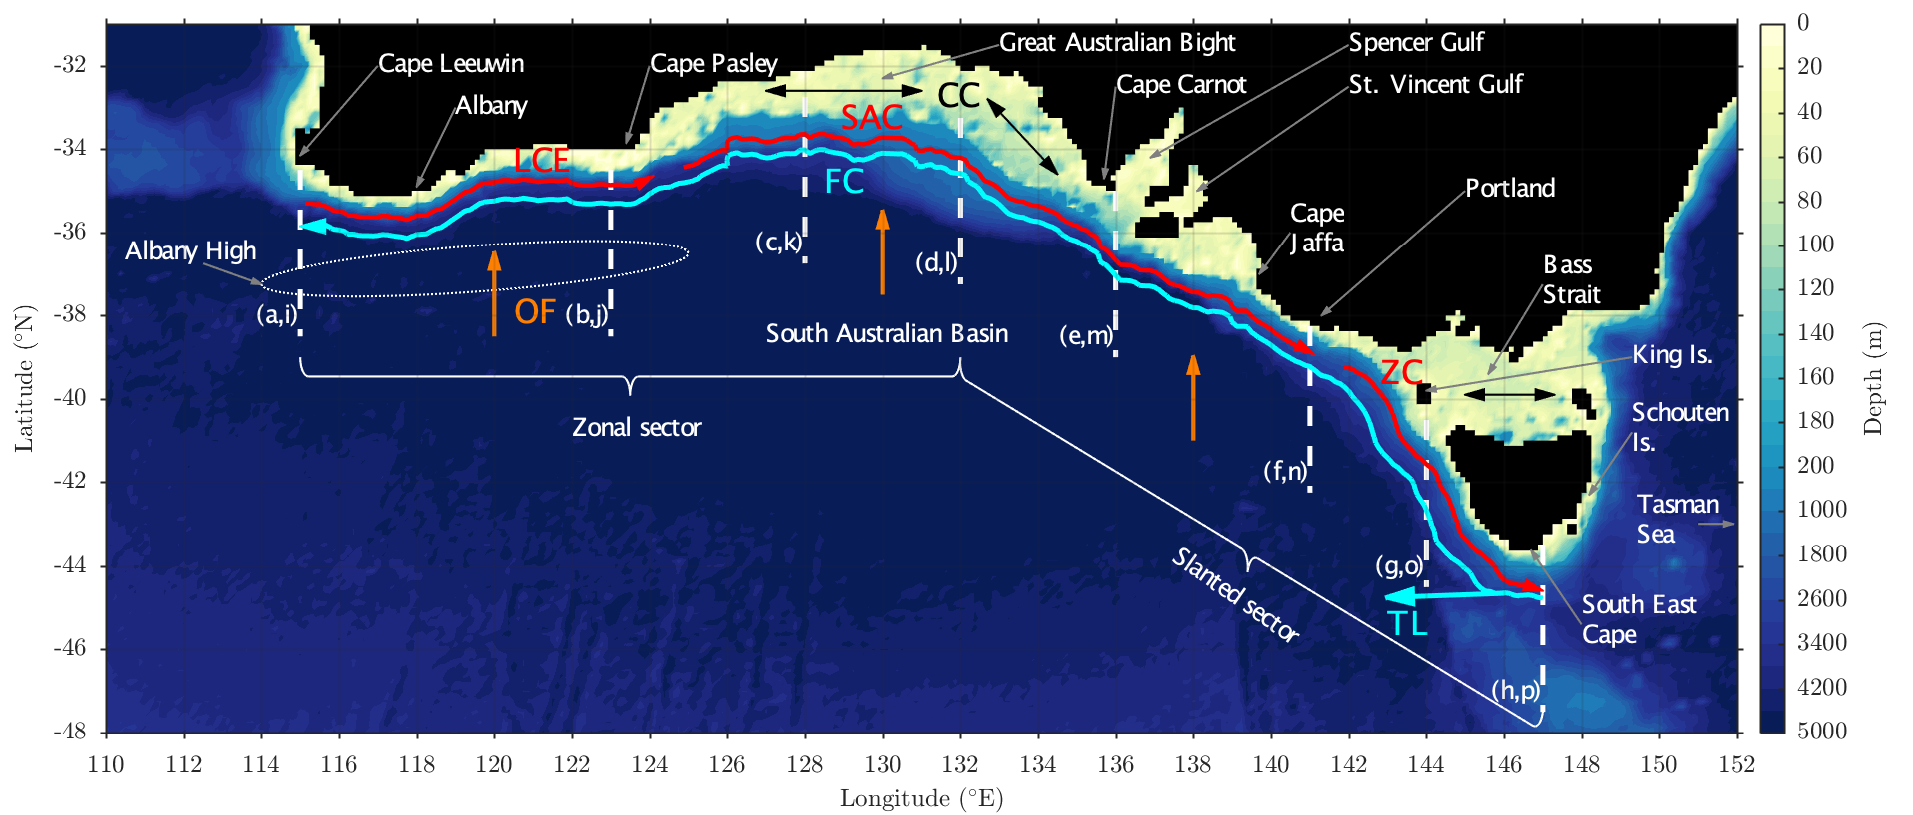
\includegraphics[width=1\textwidth, height=0.89\textheight, keepaspectratio]
{f01_fig1_.png}
\caption{\label{f01_fig1_}%
  Southern Australian bathymetry (shadings, the colour increment changes from 10 $m$ to 400 $m$ at $200\ m$) from Smith and Sandwell (1997) bin averaged onto the CARS grid, important landforms and locations (indicated by small gray arrows), major currents or flows (larger coloured arrow) and location of cross-sections for latitude versus depth plots (white dashed lines). LCE (red arrow): Leeuwin Current Extension. SAC (red arrow): South Australian Current. ZC (red arrow): Zeehan Current. FC (cyan arrow): Flinders Current. TL (cyan arrow): Tasman Leakage. OF (orange arrows): onshore flows. CC (black arrows): coastal currents.}
\end{figure}

\citet{Ridgway2004} proposed a naming convention for the surface circulation over the shelf break: (1) South of Australia, the poleward Leeuwin Current pivots anticlockwise around Cape Leeuwin (\ang{115}E) then continues eastward until Cape Pasley (\ang{124}E), the western edge of the Great Australian Bight, and is often referred to as the Leeuwin Current Extension (\citeauthor{Ridgway2004} \citeyear{Ridgway2004}, \citeauthor{Batteen2007} \citeyear{Batteen2007}); (2) The South Australian Current emerges within the Great Australian Bight and flows over the shelf break eastward then south-eastward out of the Bight, past the shallow Spencer and St.\,Vincent Gulfs, and as far south as Portland (\ang{141}E); (3) The Zeehan Current forms west of the Bass Strait, flows poleward along the western Tasmanian shelf and tips eastward around South East Cape (\ang{147}E). 
\citet{Middleton2002} described the slope circulation underneath and south of these shelf break currents. The Flinders Current flows westward from South East Cape to Cape Leeuwin. The Flinders Current has a larger width and depth range and flows in the opposite direction to the shelf break currents.

The topography of the continental margin displays varying steepness (Fig.\,\ref{f01_fig1_}). Changes in steepness mainly occur across the Great Australian Bight, delimited by Cape Pasley and Cape Carnot. Inside the Great Australian Bight, the shallow shelf is wider and the continental slope is less steep, especially on the eastern side of the Bight where isobaths between \SI{200}{\meter} and \SI{2000}{\meter} are widely spaced. The open, shallow shelf in the Bass Strait provides a connection between the South Australian Basin and the Tasman Sea. These shallow shelf regions provide a wide platform for shallow coastal currents to exist and interact with the shelf break currents. Outside these regions, the continental margin is characterised by a narrow shelf and steep slope giving a sharp shelf break. 

The orientation of the margin shifts from zonal to slanted moving eastward along the coast. The Leeuwin Current Extension and the South Australian Current flow approximately zonally until the eastern Great Australian Bight near \ang{132}E. The South Australian Current then flows along a northwest-to-southeast slant and the Zeehan Current flows approximately meridionally before it tips around South East Cape. The Leeuwin Current Extension, the South Australian Current and the Zeehan Current together form a continuous surface flow that we call the Shelf Break Currents (SBC). We refer to the ``zonal sector'' of the SBC as the flow west of \ang{132}E where the shelf break is approximately zonal, and the ``slanted sector'' as the flow east of \ang{132}E. The westward flows offshore and beneath the SBC are referred to as the Flinders Current (FC).

\subsection{The Shelf Break Currents} \label{The Shelf Break Currents}
Evidence that the Leeuwin Current rounds Cape Leeuwin and continues eastward into the Great Australian Bight is widespread. These include observations of pelagic and demersal (living close to the floor) fauna of tropical origin being found in the Great Australian Bight \citep{Garrey1981}, satellite temperature observations \citep{Legeckis1981} and estimates of steric height along the eastern Indian Ocean \citep{Godfrey1985} indicating warm waters that follow the shelf break around Cape Leeuwin and continue eastward into the Bight. The warm and relatively high salinity Leeuwin Current Extension can reach speeds greater than \SI{1}{\meter\per\second} over the \SI{200}{\meter} isobath \citep{Cresswell1993} and has a mean speed of \SI{0.5}{\meter\per\second} down to \SI{250}{\meter} along the upper slope \citep{Cresswell2004}. The Leeuwin Current Extension is periodically weakened (enhanced) by large anticyclonic eddies (small cyclonic eddies) in the region between Cape Leeuwin and Albany, as shown from surface drifter track measurements \citep{Godfrey1986} and an eddy tracking study \citep{Cresswell2004}.

The South Australian Current contains warm and very high salinity waters originating from the centre of the Great Australian Bight \citep{Rochford1986} and the Spencer and St.\,Vincent's Gulfs \citep{Godfrey1986} which flow south-eastward over the shelf break to the western Bass Strait \citep{Ridgway2004}. The South Australian Current can reach speeds of \SI{50}{\centi\meter\per\second} down to \SI{200}{\meter} along the shelf break \citep{Middleton2007}.

The Zeehan Current is a poleward current found over the western shelf break of Bass Strait and the western and southern shelf breaks of Tasmania  \citep{Baines1983,Thompson1983}. It is a relatively warm and salty current, fed by the South Australian Current, with current speeds reaching \SI{40}{\centi\meter\per\second} down to \SI{300}{\meter} \citep{Ridgway2007}. Near the southern tip of Tasmania, the Zeehan Current meets the counter-flowing East Australian Current Extension, which flows poleward along the eastern shelf break of Tasmania and pivots westward towards South East Cape \citep{Cresswell2000,Oliver2016}.

\subsection{The Deep-Ocean Circulation} \label{The Deep-Ocean Circulation}
The FC is the northern branch of the south-eastern extension of the Indian Ocean subtropical gyre \citep{Hufford1997, McCartney2007}. The FC flows westward from south of Tasmania to the south-west corner of Australia and is found between the surface and \SI{2000}{\meter} \citep{Middleton2002}. The FC is located beneath the SBC along the continental slope and extends to the sea surface south of the SBC\@.
Observational data show the FC strengthens and shoals east to west with a mean speed of \SI{4}{\centi\meter\per\second} near \SI{1000}{\meter} depth west of Tasmania, \num{3}--\SI{7}{\centi\meter\per\second} between \num{500} and \SI{900}{\meter} near Portland \citep{Middleton2007}, and \SI{20}{\centi\meter\per\second} between \num{400} and \SI{600}{\meter} near Albany \citep{Cresswell1993}.

\citepos{Middleton2002} numerical experiments showed permanent positive wind-stress curl in the South Australian Basin leads to a regional northward barotropic Sverdrup transport that is deflected westward along the southern Australian margin. It is worth noting that the Sverdrup theory cannot explain the northwestward-flowing part of the FC along the slanted coast (\ang{132}E and \ang{146}E) and particularly west of Tasmania, because it is along an eastern boundary \citep{McCreary1981,McCreary1991} and would be eliminated by the offshore propagation of Rossby waves \citep{Anderson1975}. It is therefore likely that the slanted part of the FC (as opposed to the zonal FC from \ang{132}E to Cape Leeuwin) is maintained by another mechanism.

In addition to the broad, northward Sverdrup flow, the FC is fed by narrower inflows. \citepos{McCartney2007} transport field derived from hydrographic and direct-velocity measurements show a transport starting to feed into the FC near the St.\,Vincent and Spencer Gulfs via two streamlines south of the FC that originate from the Antarctic Circumpolar Current. The eastward streamlines turn anti-clockwise south of the Great Australian Bight and accelerate the FC westward\@.

The anticlockwise circulation is likely linked to the large eddy variability west of the Great Australian Bight which was measured in a number of observational studies \citep{Cresswell1993,Godfrey1986,Ridgway2004}. A sea-surface height summer average \citep{Middleton2003} revealed the "Albany High" \citep{Middleton2007}, a large quasi-stationary anti-cyclonic eddy centred off Albany. \citepos{McCartney2007} work coincides well
with \citepos{Middleton2007} study, where the FC is the northern westward-flowing arm of the Albany High and the eastward-flowing streamlines are the southern eastward arm of the Albany High. We define the onshore flows
feeding into the FC to include both the large-scale Sverdrup flow and recirculating flow from the Albany High.

A further potential source of water to the FC is the Tasman Leakage, which carries water from the Pacific Ocean around south of Tasmania (Fig.\,\ref{f01_fig1_}). The FC is often referred to as an extension of the Tasman Leakage because part of it flows northwestward and then westward along the coast \citep{Feng2016,Middleton2002,Rosell-Fieschi2013} although most of the Tasman Leakage flows westward away from the shelf into the interior of the South Australian Basin \citep{Speich2002,vanSebille2012,vanSebille2014}.

\subsection{Present Research} \label{Present Research}
Understanding the structure and the water transport of these boundary currents is essential as they constitute a platform for carrying Indian Ocean waters from the Leeuwin Current eastward via the SBC, and Pacific Ocean waters from the Tasman Leakage south of Tasmania westward via the FC\@. 
Yet, the currents are known only from drift tracking measurements \citep{Godfrey1986,Cresswell2004}, cross-shore sections \citep{Cresswell1993}, sea surface height and sea surface temperature maps inferred from satellite data \citep{Legeckis1981,Ridgway2004} and high-resolution model experiments \citep{Middleton2002,Middleton2003,Cirano2004,Batteen2009}. While these studies provide insight into parts of the circulation, summarised in \citepos{Middleton2007} review, there is no comprehensive analysis of the three-dimensional structure and transport budget of the boundary circulation as a whole. In particular, the coupling between the SBC and the FC is still poorly understood. In the present paper, we provide the first three-dimensional geostrophic velocity field along Australia's southern boundary purely from observations, and support these results with a parallel analysis of a high-resolution model simulation.

In this study we consider the SBC and the FC as a system of currents and provide a complete description of their transport and the exchanges between them, following \citepos{Furue2017} methodology that was applied to the Leeuwin Current System along western Australia. The approach we take is to
\begin{itemize}
   \item examine the climatological, long-term mean, three-dimensional structure of the currents reconstructed from both a high-resolution gridded hydrography and an eddy-resolving ocean general circulation model forced by a seasonally-varying atmospheric climatology
   \item determine the annual-mean transport of the SBC and the FC as they travel zonally along the south coast of Australia, and the lateral transports feeding into the SBC and into the FC, and the vertical transport exchanges between the SBC and FC
   \item examine the coupling between the SBC and the FC in the annual-mean and present an overview of the currents' seasonality.
\end{itemize}
Here, we propose that the circulation in the southern Australian domain, comprising the SBC, the FC, the coastal currents (over the shallow shelf) and the onshore flows (from the ocean interior), be known as the Southern Australia Current System.

The next section provides a description of the datasets (Section~\ref{Datasets}), the derivation of mass-conserving geostrophic velocities (Section~\ref{Geostrophic velocity derivation}), the volume definition of the SBC and FC (Section~\ref{SBC and FC definition}), and the derivation of a Southern Australia Current System transport budget (Section~\ref{Transport budget derivation}). Section~\ref{Results and Discussion} presents the results where the structure of the system is described in Section~\ref{Southern Australia Current System Structure}, the transport budget of the system is described in Section~\ref{Southern Australia Current System Transport Budget} and the coupling between the SBC and the FC is described in Section~\ref{SBC and FC coupling}. Finally, Section~\ref{Summary} summarizes the analysis and presents a closing discussion in Section~\ref{Closing discussion}.

\section{Methodology} \label{Methodology}
\subsection{Datasets} \label{Datasets}
CARS-Aus8, which we simply call CARS, is a 1/8\dg-resolution climatology of ocean temperature and salinity around Australia gridded over 79 vertical levels (\citeauthor{Ridgway2002} \citeyear{Ridgway2002}; \url{http://www.marine.csiro.au/atlas/}). These levels are distributed over \SI{5500}{\meter} depth with thin levels in the upper \SI{100}{\meter} depth and thicker levels with increasing depth. The density of observations fed into CARS is high near the coast due to a large number of hydrographic measurements there \citep{Ridgway2002}. The density decreases offshore but still provides a reasonable amount of approximately spatially uniform observations due to data collected by the Argo array. The ``Aus8'' version of CARS was updated with more recent observations in early 2013 (see \citeauthor{Duran2015} \citeyear{Duran2015} and \url{http://www. marine.csiro.au/atlas/} for more details). Hydrographic profiles are mapped onto the grid through an adaptive four-dimensional interpolation technique which differs from other interpolation methods as it considers land barriers and varying topography over continental margins \citep{Ridgway2002}. Hence the interpolation technique better incorporates coastal flow structures over continental margins \citep{Ridgway2002}. For example, in the ocean interior, the interpolation technique uses a weighted least squares quadratic filter (loess filter, \citeauthor{Cleveland1988} \citeyear{Cleveland1988}) which selects nearby observations within a circle. Near the coast, in regions of shallower bathymetry, the loess filter captures data within an ellipse elongated along the isobaths. This interpolation technique narrows the data selection across the isobaths and is essential to resolve boundary currents, which are strongly constrained by topography. Due to these properties, the coastal currents are revealed in our geostrophic calculations (see Section \ref{Geostrophic velocity derivation}). The interpolation technique also purposefully creates artificial ocean data underneath the bathymetry to allow the end-user to apply their own topography mask. In the present work we choose the 2-minute (1/30\dg~resolution) version of the \citet{Smith1997} bathymetry bin-averaged onto the CARS grid. In the temporal direction, annual and semi-annual harmonics are determined by fitting at each grid point. In the present study, we use only the annual-mean component.

\citet{Ridgway2002} validated CARS against independent data and found that CARS consistently agrees with satellite and in-situ sea surface temperature products and represents the general features of the annual amplitude and phase found in in-situ data (for the seasonal variability). Salinity fronts were much better represented in CARS than in another traditional climatology, particularly in boundary current regions. The uncertainty maps indicate that in CARS the sea surface temperature over the whole Australasia is within the $\pm$0.5 $^{\circ}C$ range \citep{Ridgway2002}. Within this difference pattern, there are both coherent large-scale features as well as more intense small-scale structures near the shelf. Near the shelf, they found that inappropriately short spatial scales occur when the observations fed into CARS are heavily non-spatially uniform and form clusters of close-packed data separated by data poorer or voided areas. These tend to allow the formation of inappropriately short spatial scales from one cluster to the next in areas that have relatively little data.

To include the Ekman transport in the transport budget analysis of CARS, we use the wind stress from ERA-Interim \citep{Dee2011} averaged over 2003--2012. We choose a period corresponding to the final decade of CARS sampling when the number of observations in the upper \SI{2000}{m} is dramatically increased due to the launch of the global Argo array in 2004. In general, ERA-Interim winds are somewhat stronger between 30 and 60\dg S than satellite-based data from QuikSCAT \citep{Chaudhuri2013}.

MOM01-75z, which we simply call MOM01 in this study, is a 1/10\dg-resolution ocean model using the MOM5 code \citep{Griffies2012} and providing non-assimilated temperature, salinity and velocity fields gridded over 75 vertical levels \citep{Stewart2017}.
The model is global and forced by CORE2-NYF, a repeated climatological annual cycle of sea-surface atmospheric forcing with six hourly synoptic variability \citep{Large2009}.
MOM01 is forced under this cycle for 108 years and we select the last 7 years to produce our equilibrated mean ocean state. 

We will use the temperature and salinity fields in MOM01 to calculate the geostrophic velocity (see Section~\ref{Geostrophic velocity derivation}). On one hand, we will compare the geostrophic velocity from CARS to the full model velocity from MOM01. On the other hand, we will compare the CARS transport budget derived from geostrophic velocity to the MOM01 transport budget derived from geostrophic velocity and to the MOM01 transport budget calculated from full model velocity. The comparison of MOM01 geostrophic transport budget with the MOM01 full model transport budget will serve to test the method we use to derive geostrophic velocity. A short discussion of this test is in Section\,\ref{Southern Australia Current System Transport Budget}.

In Section\,\ref{Southern Australia Current System Structure} we find that CARS shows some minor artificial fragmentation in the currents which we briefly discussed above citing \citet{Ridgway2002}. Our high resolution model, however, produces a coherent current system. In addition, the prescribed climatological forcing applied to the model results in a  numerical simulation of a mean and seasonal cycle that is well suited for comparison with those from the CARS observational climatology.
We note that the winds in CORE2-NYF, which are based on the National Centers for Environmental Prediction (NCEP) reanalysis, are generally stronger than those from satellite-based data from QuikSCAT \citep{Large2009}. CORE2-NYF winds are in good agreement with ERA-Interim winds, although in the southern hemisphere, the westerlies are slightly stronger in ERA-Interim, particularly around 50\dg S \citep{Chaudhuri2013}.

\subsection{Geostrophic velocity derivation} \label{Geostrophic velocity derivation}
The varying flow structures of the Southern Australia Current System greatly reduce our ability to test different depth levels of no-motion to derive geostrophic velocities. Since the FC can extend as deep as \SI{2000}{\meter} \citep{Middleton2002}, we choose a reference depth of $z\sub{ref} = \SI{-2000}{\meter}$, which is also the depth limit of Argo observations. We note that the annual-mean density field in CARS and MOM01 agree reasonably well, except near Albany where CARS shows lighter surface densities, which would result in a higher Albany High (not shown).

To compute geostrophic velocities in regions shallower than the reference depth, we apply the Helland-Hansen method \citep{Helland-Hansen1934,Fomin1964}. This method states that velocities at the bottom of a land portion shallower than the reference depth are zero. We first compute geostrophic velocities referenced to the surface and then remove a vertically-uniform velocity field that cancels out the geostrophic velocities at the reference depth in the ocean interior or at the sea bottom over the margin; hence

\begin{equation}
\Vec{v\sub{g}^{*}} = \Vec{v\sub{0}} - \Vec{v\sub{0}}(z=z\sub{HH}),
\end{equation}
%
where $z \in [\SI{-2000}{\meter}, 0]$ is the local depth, $z\sub{HH} = \max(z\sub{ref},z\sub{b})$ is a depth that corresponds to the shallowest level between $z\sub{ref}$ and the local sea bottom depth $z\sub{b}(x,y)$, $\Vec{v\sub{0}}=(u\sub{0},v\sub{0})$ are the geostrophic velocities referenced to the surface and $\Vec{v\sub{g}^{*}}$ are the geostrophic velocities from the Helland-Hansen method.

To account for the wind effect at the surface we calculate the Ekman drift $\Vec{V\sub{ek}}$ (\si{\square\meter\per\second}) as

\begin{equation}
\Vec{V\sub{ek}} = -\Vec{k} \times \frac{\boldsymbol{\tau}}{f\rho\sub{0}},
\end{equation}
%
where $\Vec{k}$ is an upward pointing unit vector, $\boldsymbol{\tau}=(\boldsymbol{\tau}^{x},\boldsymbol{\tau}^{y})$ is the wind stress, $f$ is the Coriolis parameter and $\rho\sub{0}$ is a constant mean density. Note that in the geostrophic calculation, we assume that the bottom is slippery and therefore there is no Ekman transport at the bottom.

A drawback of the Helland-Hansen method is that it produces large vertical flows across the sea bottom over the margin, which introduces error in three-dimensional transport budgets. These cross-bottom leaks are evident from high divergence values in the depth-integrated velocity field, $\nabla\cdot\Vec{V}^{*}$ (not shown). This depth-integrated velocity field $\Vec{V}^{*}=\Vec{V\sub{g}^{*}}+\Vec{V\sub{ek}}$ is the sum of contributions from both geostrophy and Ekman drift and is defined as

\begin{equation}
\Vec{V}^{*} = \int_{z\sub{HH}}^{0}\Vec{v\sub{g}^{*}}\ dz + \Vec{V\sub{ek}}.
\end{equation}
%
To eliminate this deficiency, we apply the Zero-Divergence method described in \citet{Furue2017}. Here, we remove a second barotropic velocity field $\Vec{V\sub{d}}=\nabla\phi$ from $\Vec{V}^{*}$ such that $\nabla\cdot(\Vec{V}^{*}-\nabla\phi)=0$, so that $\phi$ satisfies the Poisson equation

\begin{equation}
\nabla^{2}\phi = \nabla\cdot\Vec{V}^{*}.
\end{equation}
%
We solve the above equation by setting a no-flow condition on $\Vec{V\sub{d}}$ everywhere at the solid land and open ocean boundaries except along the southern open ocean boundary. At the southern boundary we set $\phi=0$ there to allow for a net inflow or outflow of $\Vec{V\sub{d}}$ to compensate for the total divergence $\iint\nabla\cdot\Vec{V}^{*}\,dx\,dy$. In order to ensure the impact of that weak artificial flow over the Southern Australia Current System is minimal, we set the open boundary \ang{2} south of our domain, along \ang{50}S. The resulting adjusted geostrophic field $\Vec{v\sub{g}}$ is expressed as

\begin{equation}
\Vec{v\sub{g}} = \Vec{v\sub{g}^{*}} - \frac{\Vec{V\sub{d}}}{-z\sub{HH}},
\end{equation}
%
where $\nabla\cdot\Vec{V}=\nabla\cdot(\int_{z\sub{HH}}^{0}\Vec{v\sub{g}}\ dz + \Vec{V\sub{ek}})=0$ everywhere including over the continental shelf and slope.

\subsection{SBC and FC definition} \label{SBC and FC definition}
To calculate the Southern Australia Current System transport budgets we define two control volumes, one surrounding the SBC and the other surrounding the FC\@. These boundaries are defined by visually inspecting meridional sections in CARS. We then apply the same boundaries to the mean field in MOM01 to keep consistent volumes in our calculations. 

We first inspect meridional sections at the locations shown in Fig.\,\ref{f01_fig1_} (black dashed lines) to find the vertical structure of the currents and their position relative to the margin (Fig.\,\ref{f02_fig1_}a-h). The reader can also compare the CARS sections with the MOM01 sections which use the full model velocity (Fig.\,\ref{f02_fig1_}i-p). Since the orientation of the coastline varies as the currents progress zonally, we consider both zonal and meridional flow components to help identify the currents. Therefore, in Fig.\,\ref{f02_fig1_} we present the zonal component as shading and the meridional component as contours. The longshore currents can be clearly identified in the zonal velocity up until Cape Carnot at \ang{136}E (Fig.\,\ref{f02_fig1_}e). Further east, the meridional component of flow helps to identify the currents.

While the SBC are relatively narrow, thin and well contained along the shelf break, the FC is wider and thicker with a core position that varies more than the SBC\@. We define here an \enquote{offshore FC}
south of the SBC, centered at the surface and extending downward as deep as \SI{2000}{\meter} (Fig.\,\ref{f02_fig1_}b,c,d,f,h), and
a \enquote{slope FC} at sub-surface level centered at \SI{600}{\meter} underneath the SBC and adjacent to the slope (Fig.\,\ref{f02_fig1_}b,c,e,g). The slope FC forms a clearer separate core from the offshore FC in the numerical model (Fig.\,\ref{f02_fig1_}i-o).
Hence, the SBC and FC volumes can be defined by separating the water column into an upper layer that contains the whole SBC and the upper offshore FC, and a lower layer that contains the slope FC and the lower offshore FC\@. The horizontal interface $z\sub{int}$ between the upper and lower layers is therefore the SBC bottom boundary. We choose $z\sub{int} = \SI{-250}{\meter}$ (Fig.\,\ref{f02_fig1_}, blue line) as this level is generally very close to, or within, the \num{0} to \SI{4}{\centi\meter\per\second} eastward velocity range beneath the SBC.
%
\begin{figure}[p]
\centering
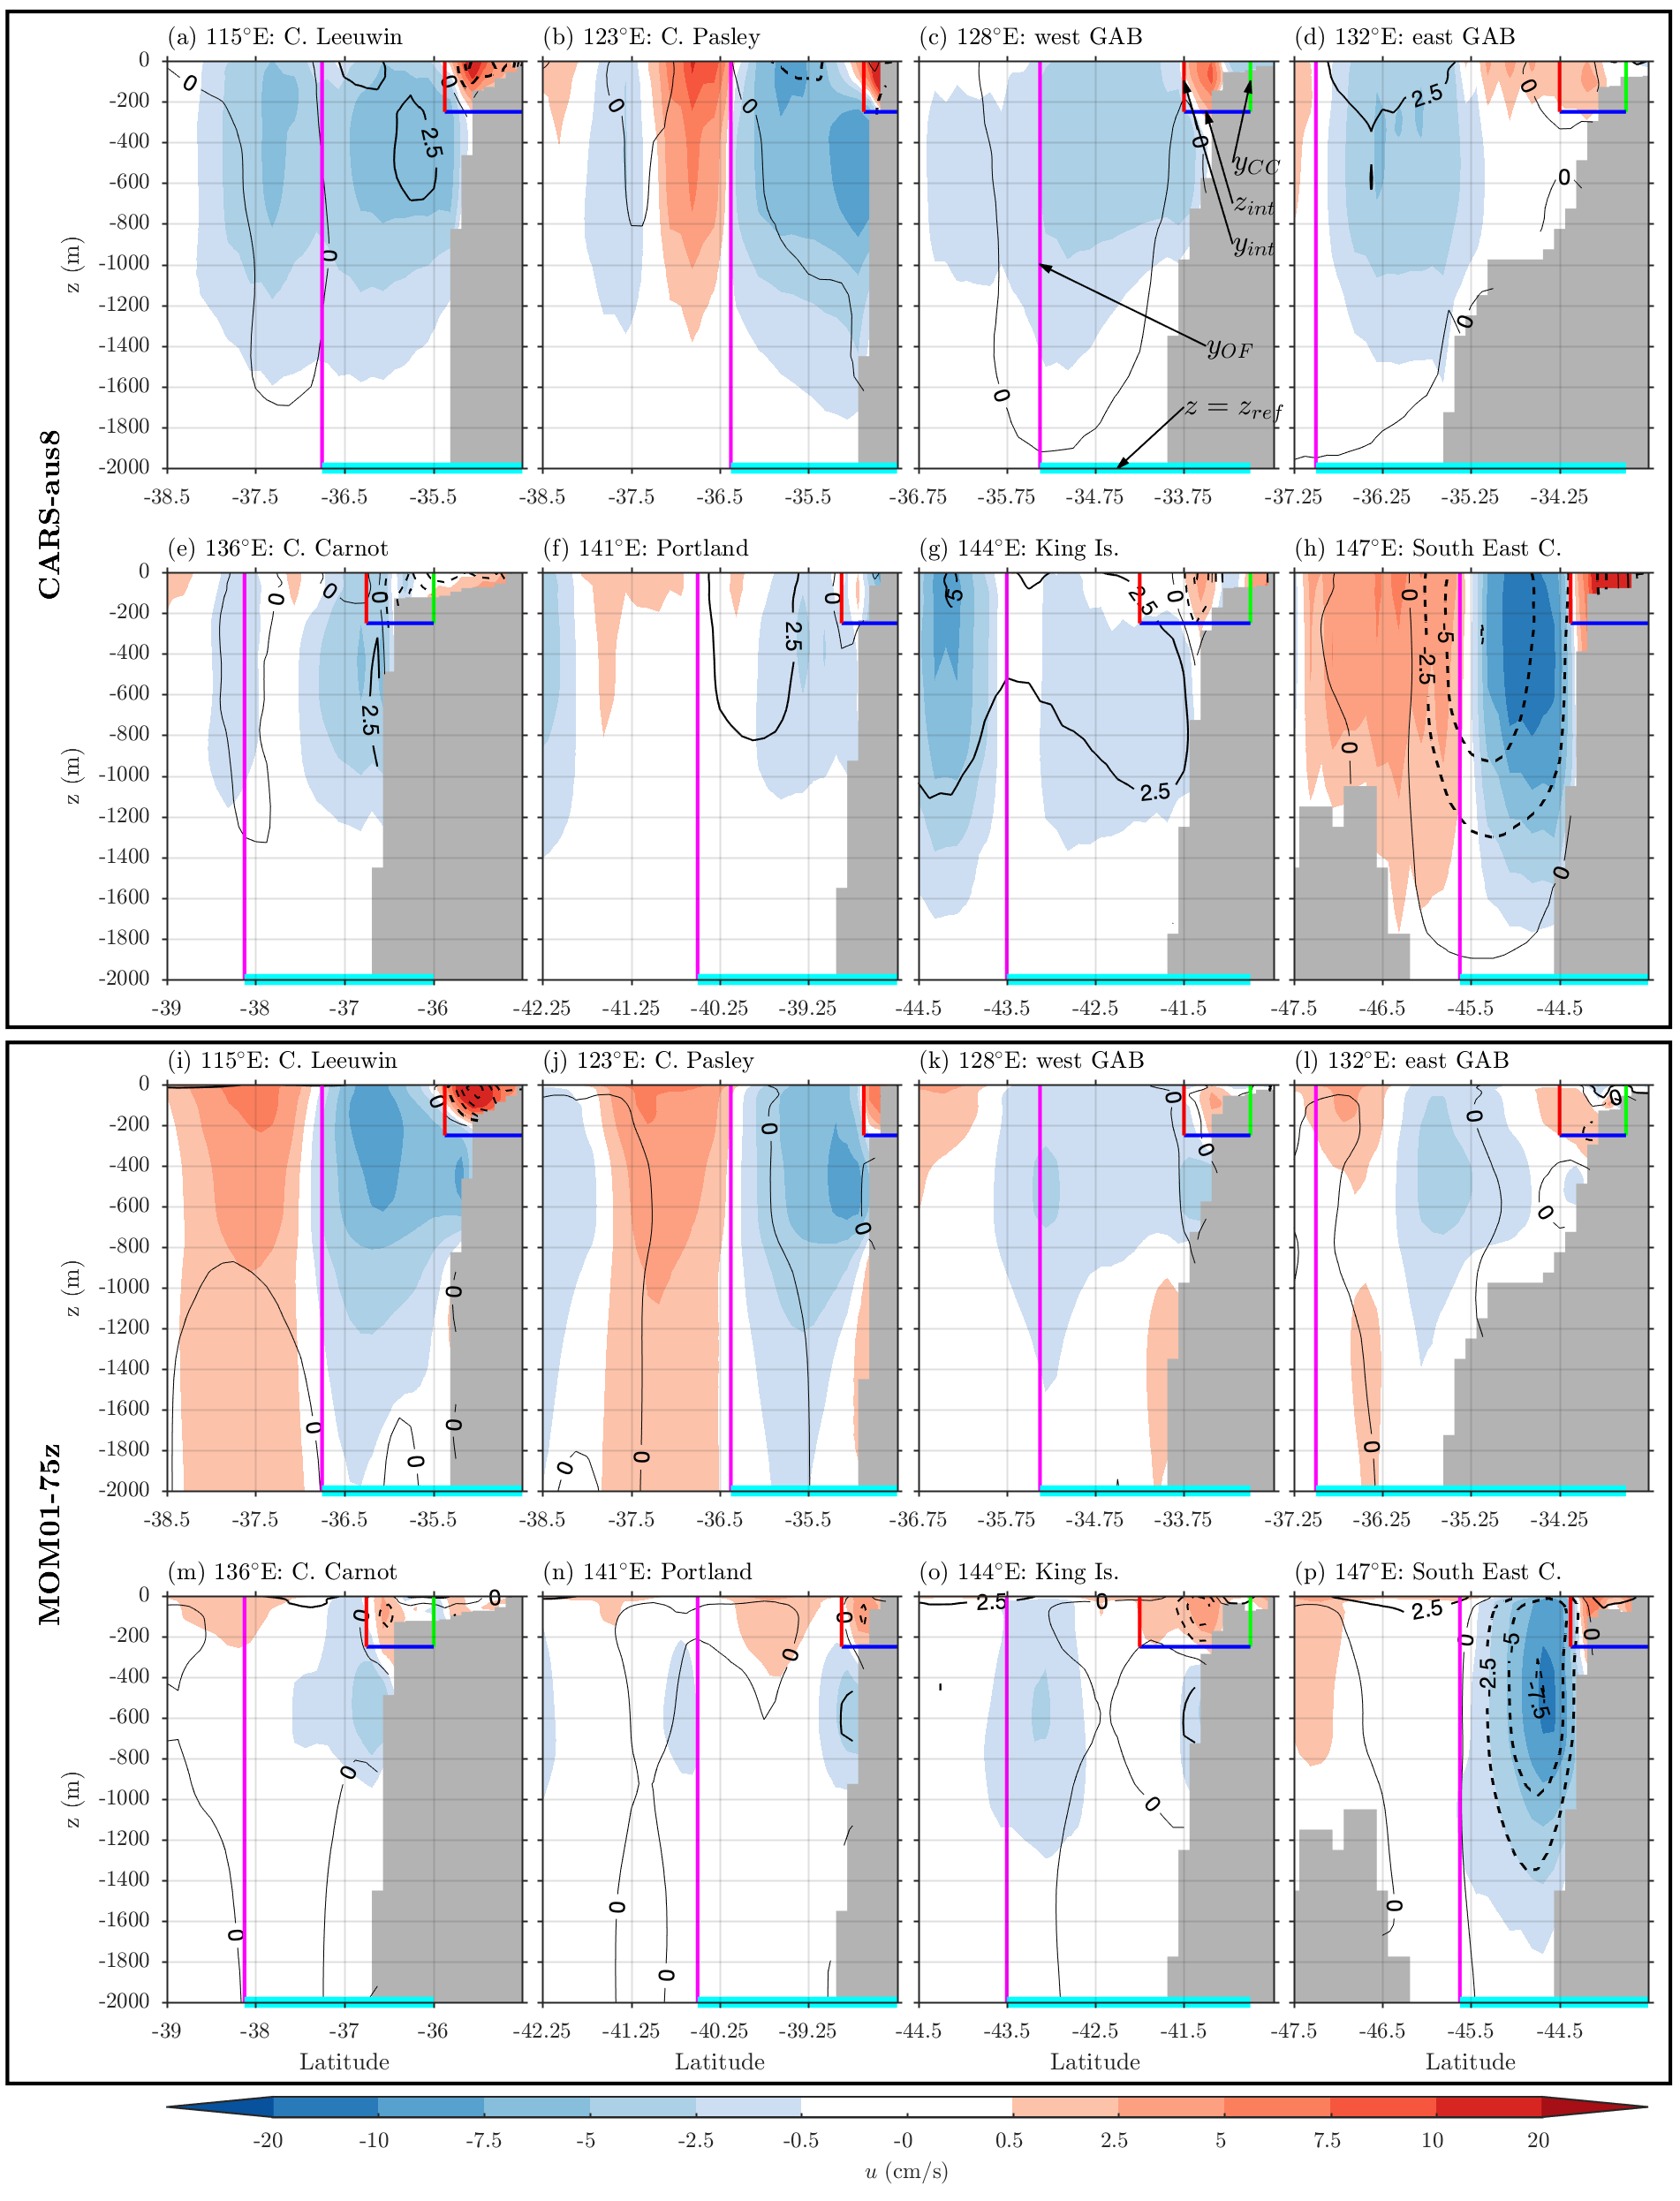
\includegraphics
[width=\textwidth, height=0.89\textheight, keepaspectratio]
{f02_fig1_.png}
\caption{\label{f02_fig1_}%
  Meridional sections along southern Australia of (a-h) geostrophic velocities in CARS and (i-p) actual velocities in MOM01. Zonal geostrophic velocities $u\sub{g}$ in CARS (actual zonal velocities in MOM01) in \si{\centi\meter\per\second} (shadings, non-monotonic scale) and meridional geostrophic velocities $v\sub{g}$ in CARS (actual meridional velocities in MOM01) in \si{\centi\meter\per\second} (contours, every \SI{2.5}{\centi\meter\per\second}, thick solid lines show positive values, thick dashed lines show negative values, thin solid lines show zero contour). Boundaries of the SBC and FC as follows: $y\sub{CC}$ (green) is the SBC north boundary; $z\sub{int}$ (blue) is the SBC bottom boundary and the FC top boundary; $y\sub{int}$ (red) is the SBC south boundary and the FC north boundary; $y\sub{OF}$ (magenta) is the FC south boundary; $z\sub{ref}$ (thick cyan) is the FC bottom closed boundary at the reference depth.}
\end{figure}


We define the northern and southern boundaries of the SBC and FC by inspecting maps of CARS velocities integrated in the upper layer $\Vec{V\sub{up}}$ (Fig.\,\ref{f03_fig1_}a) and velocities integrated in the lower layer $\Vec{V\sub{low}}$ (Fig.\,\ref{f03_fig1_}b). $\Vec{V\sub{up}}$ is the integral of geostrophic velocities from the surface to $z\sub{int}$ plus the Ekman drift and $\Vec{V\sub{low}}$ is the integral of geostrophic velocities from $z\sub{int}$ to $z\sub{ref}$. These are depth integrated velocity fields which can be regarded as transports per unit width in \si{\square\meter\per\second},
%
\begin{equation} \label{eq:1}
\Vec{V\sub{up}}(x,y) = \int_{z\sub{int}}^{0}\Vec{v\sub{g}}\ dz + \Vec{V\sub{ek}}
\end{equation}
%
\begin{equation} \label{eq:2}
\Vec{V\sub{low}}(x,y) = \int_{z\sub{ref}}^{z\sub{int}}\Vec{v\sub{g}}\ dz.
\end{equation}
%
Note that $\Vec{V\sub{up}}$ and $\Vec{V\sub{low}}$ from MOM01 are shown in Fig.\,\ref{f03_fig1_}c,d. In this case we have used the full model velocity in equations \ref{eq:1} and \ref{eq:2} rather than the sum of geostrophic and Ekman components from the model. A comparison of the MOM01 full model velocity with the MOM01 geostrophic and Ekman velocity shows that the full model velocities in the SBC and FC are generally stronger than the sum of the geostrophic and Ekman components (not shown). Therefore the MOM01 full model longshore transport for the SBC and the FC will be stronger than the MOM01 geostrophic longshore transport (see Section\,\ref{Southern Australia Current System Transport Budget}).
%
\begin{figure}[p]
\centering
\includegraphics%
[width=\textwidth, height=0.92\textheight, keepaspectratio]
{f03_fig1_.png}
\caption{\label{f03_fig1_}%
  Depth integrated (a,b) geostrophic velocities in CARS and (c,d) actual velocities in MOM01, showing the velocity field (directional plot) and the zonal component (shadings, non-monotonic scale) in \si{\square\meter\per\second} (ie. transport per unit width). The fields are integrated from (a,c) the surface to \SI{-250}{\meter} and from (b,d) \SI{-250}{\meter} to \SI{-2000}{\meter}. In CARS, (a) shows the sum of geostrophic velocities and Ekman velocities and (b) shows geostrophic velocities only. Boundaries of the SBC and FC as follows: $y\sub{CC}$ (green with black outline) is the SBC north boundary; $y\sub{int}$ (red with black outline) is the SBC south boundary and the FC north boundary; $y\sub{OF}$ (magenta with black outline) is the FC south boundary; $z\sub{int}$ area is the surface bounded by $y\sub{int}$ at south and the slope at north.}
\end{figure}

We present in Fig.\,\ref{Diagram_V3} a three-dimensional schematic diagram of the Southern Australia Current System to understand the exchanges in the transport budget. This schematic illustrates the transport of the eastward SBC ($U_{SBC}$ thick light blue arrow) and the westward FC ($U_{FC}$ thick light yellow arrows), which includes the slope FC below the SBC, and the upper and lower parts of the offshore FC. Inward/outward transports into or out of the longshore SBC or FC are indicated as thin coloured arrows. Here, an increase in SBC transport can be supplied from three sources: southward horizontal inflow from the coastal currents ($V_{CC}$ thin green arrows), northward horizontal inflow from the offshore FC near the surface ($V_{SBC}$ thin red arrows), and upwelling from the slope FC ($W_{SBC}$ thin blue arrows). Similarly, an increase in FC transport can be supplied by three sources: southward horizontal inflow from the SBC into the surface FC ($V_{FC}$ thin red arrows), downwelling from the SBC into the slope FC ($W_{FC}$ thin blue arrows), northward flow from the ocean interior into the upper or lower part of the offshore FC ($V_{OF}$ thin magenta arrows).
%
\begin{figure}[hbp]
\centering
\includegraphics%
[width=\textwidth, height=0.89\textheight, keepaspectratio]
{Diagram_V3.pdf}
\caption{\label{Diagram_V3}%
  Southern Australia Current System transport budget schematics. The SBC transport is shown as a thick light blue arrow, the offshore FC transport and the slope FC as thick light yellow arrows. The shallow coastal currents are shown as a black two-ways arrow. The inward/outward transports into/out of the SBC and FC are shown as thin coloured arrows. There are four of such exchanges: the horizontal transport between the coastal currents and the SBC (green arrows), the horizontal transport between the SBC and the offshore FC in the upper layer (red arrows), the vertical transport between the SBC and the slope FC (blue arrows) and the horizontal transport from the onshore flows into all the offshore FC (magenta arrows).}
\end{figure}

The boundaries forming the control volume around the SBC and around the FC are shown in the meridional sections of velocities (Fig.\,\ref{f02_fig1_}) and maps of depth integrated velocities (Fig.\,\ref{f03_fig1_}). The SBC receive contributions from the coastal currents (Fig.\,\ref{Diagram_V3}, green arrows) through a vertical face on the shallow shelf $y\sub{CC}$ (Figs.\,\ref{f02_fig1_}\,and\,\ref{f03_fig1_}, green line). They also undergo exchanges with the FC horizontally (Fig.\,\ref{Diagram_V3}, red arrows) through the vertical face $y\sub{int}$ (Figs.\,\ref{f02_fig1_}\,and\,\ref{f03_fig1_}, red line) to the south of the SBC, and vertically (Fig.\,\ref{Diagram_V3}, blue arrows) through $z\sub{int}$ (Fig.\,\ref{f02_fig1_}, blue line) at the bottom of the SBC\@. The FC undergoes equal but opposite exchanges with the SBC through $y\sub{int}$ and $z\sub{int}$\@. The FC also receives contributions from the ocean interior onshore flows (Fig.\,\ref{Diagram_V3}, magenta arrows) through a vertical face $y\sub{OF}$ (Figs.\,\ref{f02_fig1_}\,and\,\ref{f03_fig1_}, magenta line) to the south of the FC over the depth range 0 to \SI{2000}{\meter}. The onshore flows represent the northward, deep-reaching Sverdrup transport and re-circulation from the Antarctic Circumpolar Current described in Section\,\ref{The Deep-Ocean Circulation}.
Note that there is no vertical flow across the bottom of the FC as this boundary is at the reference depth $z\sub{ref}$ (Fig.\,\ref{f02_fig1_}, cyan line).

Since the SBC and FC are strongly topographically controlled, we define their northern and southern boundaries by working along two isobaths: one that best follows the SBC and another one that best follows the FC\@. In the upper layer (Fig.\,\ref{f03_fig1_}a), the SBC's northern (southern) boundary is defined as some degrees north (south) of their isobath depending on the current's cross-shore width. The FC's northern boundary is defined as the SBC's southern boundary in the upper layer and as the continental slope in the lower layer (Fig.\,\ref{f03_fig1_}b). The FC's southern boundary is defined as some degrees south of its isobath depending on the current's seaward extent. 

Since the shelf orientation varies, we increase the distance between the SBC's northern and southern boundaries when the shelf is more slanted to ensure the SBC are fully captured. West of Portland, we select the \SIadj{700}{\meter} isobath for the SBC and define $y\sub{CC}$ to be 3/8\dg~to the north and $y\sub{int}$ to be 3/8\dg~to the south. East of Portland, where the shelf break is meridional, we define $y\sub{CC}$ to be 1/2\dg~to the north and $y\sub{int}$ to be 3/4\dg~to the south of the \SIadj{700}{\meter} isobath. South of Tasmania, where the coastline is zonal, $y\sub{int}$ is 3/8\dg~to the south of the isobath again.
We remove $y\sub{CC}$ where the shallow shelf is narrow and the coastal currents are insignificant, that is anywhere outside the Great Australian Bight, the Bass Strait, the Gulfs region north of Cape Jaffa. Finally, we define the FC's southern boundary $y\sub{OF}$ by following the \SIadj{2000}{\meter} isobath. West of Portland $y\sub{OF}$ is set to be 3/2\dg~south of this isobath. Elsewhere, it is set to be 7/4\dg~south. South of Tasmania, the boundary is manually adjusted to lie at \ang{45.5}S.
The green, red and magenta curves in Fig.\,\ref{f03_fig1_} are $y\sub{CC}$, $y\sub{int}$ and $y\sub{OF}$ as defined above.

We note that MOM01 shows continuous SBC that are well incorporated into the SBC control volume (Fig.\,\ref{f03_fig1_}c). Even though CARS is a long-term climatology, it still includes some coastal eddy-like ``noise'' in the region (Fig.\,\ref{f03_fig1_}a), which is likely due to the superposition of eddies recorded at different times. Recently, \citet{Oke2018} found that the shelf off the Great Australian Bight is rich in mesoscale eddies with surface-intensified currents coherent over the water column. The eddies, which are hypothetically due to the horizontal shear associated with the SBC, are most energetic when the SBC start to seasonally weaken. In MOM01, the synoptic structure of eddies, particularly in the Leeuwin Current Extension region, is evident on transient timescales (not shown). Defining fixed boundaries around the SBC is, however, adequate, because the long-term mean boundary circulation is mostly dominated by the geostrophic flow. The SBC's jet like shape is maintained by the southward propagation of pressure anomalies coming from the Leeuwin Current System and turning eastward along the southern coast of Australia \citep{Middleton2007, Ridgway2015}. In winter, the currents are reinforced due to intensification of westerly winds and increased onshore Ekman transport \citep{Ridgway2004}. Hence, in our fixed boundary definition for the SBC, any eddies and eddy-like meandering flows crossing the boundaries will be captured as an inflow or outflow into the currents. \citet{Furue2017} also applied fixed boundaries for the Leeuwin Current System, because the Leeuwin Current, which co-exists with eddies, is also a jet-like flow.

\subsection{Transport budget derivation} \label{Transport budget derivation}
We calculate the local zonal transport within these volumes,
which we refer to as the SBC or FC transport, and the inward/outward transport across all volume boundaries which we refer to as the cross-boundary transport. The SBC transports include both geostrophic and Ekman transports. The FC transports include geostrophic and Ekman transport in the upper layer south of the SBC, and only geostrophic transports in the lower layer (slope FC and offshore FC).
We carry out the same calculations on the full (total) velocity from MOM01.
Below, we provide identities for SBC and FC that connect their longshore transports to cross-boundary exchanges. The following equations represent a transport in volume per unit time in Sverdrups (\si{Sv},  \SI[parse-numbers=false]{10^6}{\cubic\meter\per\second}).

We choose to use Cartesian coordinates, rather than coast-following, because the currents are narrow (particularly the SBC) and it is difficult to define a coast-following coordinate system that allows mass to be conserved in the transport calculation. Our approach assures mass conservation through careful selection of the grid cells in the transport budget, and capturing of all flow into and out of each cell. \ref{Reasoning for defining the SBC transport and the FC transport from their zonal transport} explains our reasoning for choosing cartesian coordinates over coast-following ones.

We first present the longshore and cross-boundary equations for the SBC\@. The following transport equations are indicated in Fig.\,\ref{Diagram_V3}. When we refer to the transport of a current (e.g. SBC), this is the full longshore transport carried by the current. Cross-shore exchanges are captured by the cross-boundary transports. For the SBC, the longshore and cross-shore transports are defined as follows. The SBC transport $\mathcal{U}\sub{SBC}$ is 

\begin{equation} \label{eq:3}
\mathcal{U}\sub{SBC}(x) = \int_{y\sub{int}(x)}^{y\sub{CC}(x)}{U}\sub{up}\ dy,
\end{equation}
%
where $U\sub{up}$ is defined by (6). Hence $\mathcal{U}\sub{SBC}$ represents the transport between $y\sub{int}$ and $y\sub{CC}$. 

The cumulative horizontal cross-boundary transports into the SBC are 

\begin{equation} \label{eq:4}
\mathcal{V}\sub{CC}(x) = \int_{x\sub{west}}^{x}\Vec{n}\sub{CC}\cdot\Vec{V}\sub{up}\ dl\sub{CC},
\end{equation}
%
\begin{equation} \label{eq:5}
\mathcal{V}\sub{SBC}(x) = \int_{x\sub{west}}^{x}\Vec{n}\sub{int}\cdot\Vec{V}\sub{up}\ dl\sub{int},
\end{equation}
%
where $x\sub{west}$ = \ang{115}E is the longitude at the western edge of the SBC, $dl\sub{CC}$ and $dl\sub{int}$ are the line elements of the curves $y\sub{CC}$ and $y\sub{int}$, respectively, from $x\sub{west}$ to $x$ and $\Vec{n}$ is a unit vector perpendicular to $dl$ and pointing into the SBC\@.
$\mathcal{V}\sub{CC}$ and $\mathcal{V}\sub{SBC}$ hence represent the horizontal cross-boundary transport across $y\sub{CC}$ (from the coastal currents into the SBC) and $y\sub{int}$ (from the offshore FC into the SBC),respectively, accumulated from $x\sub{west}$ to $x$. Positive transport values are defined to be directed into the SBC volume.

The vertical cross-boundary transport into the SBC is defined as

\begin{equation} \label{eq:6}
\mathcal{W}\sub{SBC}(x)
= \int_{x\sub{west}}^{x} \int_{y\sub{int}(x)}^{y\sub{CC}(x)} \nabla\cdot\Vec{V}\sub{up}\ dy\ dx.
\end{equation}
%
Hence $\mathcal{W}\sub{SBC}$ represents the vertical cross-boundary transport across $z\sub{int}$, from the slope FC into the SBC (positive upwards), accumulated from $x\sub{west}$ to $x$.

We now define the longshore and cross-boundary equations for the FC\@. The FC transport $\mathcal{U}\sub{FC}$ is 

\begin{equation} \label{eq:7}
\mathcal{U}\sub{FC}(x) = \int_{y\sub{OF}(x)}^{y\sub{int}(x)}{U}\sub{up}\ dy
+ \int_{y\sub{OF}(x)}^{y\sub{slope}(x)}{U}\sub{low}\ dy,
\end{equation}
%
where $U\sub{low}$ is defined by (7) and $y\sub{slope}$ is the latitude of the slope at $z\sub{int}$. $\mathcal{U}\sub{FC}$ hence represents the sum of the offshore FC transport in the upper layer (integrated between $y\sub{OF}$ and $y\sub{int}$) and the FC transport in the lower layer (integrated between $y\sub{OF}$ and the slope). The lower layer FC transport includes both the lower layer of the offshore FC and the slope FC.

The horizontal cross-boundary transport across $y\sub{OF}$, representing the input into the offshore FC from the ocean interior, is defined as

\begin{equation} \label{eq:8}
\mathcal{V}\sub{OF}(x) = \int_{x}^{x\sub{east}}\Vec{n}\sub{OF}\cdot(\Vec{V}\sub{up} + \Vec{V}\sub{low})\ dl\sub{OF},
\end{equation}
%
where $x\sub{east}$ = \ang{147} is the longitude at the eastern edge of the FC, $dl\sub{OF}$ is the line element of $y\sub{OF}$ from $x$ to $x\sub{east}$ and $\Vec{n}$ is a unit vector perpendicular to $dl$ and pointing into the FC\@. $\mathcal{V}\sub{OF}$ thus represents the upper- and lower-layer horizontal cross-boundary transport across $y\sub{OF}$ into the FC (positive into the FC) accumulated from $x$ to $x\sub{east}$. 

The other cross-boundary transports into the FC across $y\sub{int}$ and $z\sub{int}$ are equal and opposite to the corresponding cross-boundary transports of the SBC (ie. $\mathcal{V}\sub{SBC}$ and $\mathcal{W}\sub{SBC}$, respectively) and are accumulated in the opposite direction, from east to west. Hence

\begin{equation} \label{eq:9}
\mathcal{V}\sub{FC}(x) = \int_{x}^{x\sub{east}}-\Vec{n}\sub{int}\cdot\Vec{V}\sub{up}\ dl\sub{int},
\end{equation}
%
\begin{equation} \label{eq:10}
\mathcal{W}\sub{FC}(x) = \int_{x}^{x\sub{east}} \int_{y\sub{int}(x)}^{y\sub{CC}(x)} -\nabla\cdot\Vec{V}\sub{up}\ dy\ dx,
\end{equation}
%
where $\mathcal{V}\sub{FC}$ and $\mathcal{W}\sub{FC}$ represent the cross-boundary transports into the FC accumulated from $x$ to $x\sub{east}$ across $y\sub{int}$ (positive out of the SBC) and across $z\sub{int}$ (positive downwards, out of the SBC), respectively.

Finally, since both
the adjusted geostrophic plus Ekman velocities and MOM01's full velocities are mass conserving, the transports $\mathcal{U}\sub{SBC}$ and $\mathcal{U}\sub{FC}$ can also be obtained by using the Continuity equation and interpreting all the cumulative transport terms as sources and sinks. Hence,

\begin{equation} \label{eq:11}
\mathcal{U}\sub{SBC}(x) = \mathcal{U}\sub{SBC}(x\sub{west}) + \mathcal{V}\sub{CC}(x) + \mathcal{V}\sub{SBC}(x) + \mathcal{W}\sub{SBC}(x).
\end{equation}
%
\begin{equation} \label{eq:12}
-\mathcal{U}\sub{FC}(x) = -\mathcal{U}\sub{FC}(x\sub{east}) + \mathcal{V}\sub{FC}(x) + \mathcal{V}\sub{OF}(x) + \mathcal{W}\sub{FC}(x).
\end{equation}
%
We note that in equation (17), there is a negative sign in front of $\mathcal{U}\sub{FC}(x)$ because the FC transport is westward (hence negative). We calculate the terms using definitions (8)--(15)
and verify that the above equalities are satisfied at
very high accuracy (see Fig.\,\ref{Slide1_2}).

\section{Results and Discussion} \label{Results and Discussion}
This section is divided into three subsections. Firstly, we examine the annual-mean three-dimensional structure of the major currents of the Southern Australia Current System (Section~\ref{Southern Australia Current System Structure}). Secondly we analyse the transport budget from the annual-mean current transport and cross-boundary transport of the SBC and the FC (Section~\ref{Southern Australia Current System Transport Budget}). Finally, a discussion of the SBC--FC coupling in the annual-mean and in summer and autumn is presented (Section~\ref{SBC and FC coupling}).

\subsection{Southern Australia Current System Structure} \label{Southern Australia Current System Structure}
We first inspect meridional sections of mean zonal and meridional velocities in CARS and MOM01 and compare our results with those reported in the literature (Section~\ref{Shelf meridional sections}). We then describe the system from maps of depth integrated velocities in the upper layer (SBC and upper FC) and lower layer (lower FC, Section~\ref{Depth-integrated velocity maps}). Finally we examine the upper slope vertical flows between the SBC and the slope FC (Section~\ref{Vertical flows in MOM01}).

\subsubsection{Shelf meridional sections}\label{Shelf meridional sections}
In the cross-sections, the structure and speed of the Leeuwin Current Extension, the western SBC flow in the Cape Leeuwin and Cape Pasley sections, is generally in good agreement between CARS (Fig.\,\ref{f02_fig1_}a,b) and MOM01 (Fig.\,\ref{f02_fig1_}i,j). The current shrinks and weakens moving east and flows over the shelf break between the surface and \SI{250}{\meter} which agrees well with estimates from \citet{Cresswell2004} and \citet{Cresswell1993}. They reported instantaneous speed records up to \num{50} and \SI{100}{\centi\meter\per\second} which is in good agreement with MOM01 which showed 5-days average Leeuwin Current Extension speed greater than \SI{50}{\centi\meter\per\second} in autumn (not shown).

The South Australian Current, the central SBC flow in the Great Australian Bight and Cape Carnot sections, weakens as it flows eastward across the Bight in CARS (Fig.\,\ref{f02_fig1_}c,d) and reverses to become a south-westward flow off Cape Carnot (Fig.\,\ref{f02_fig1_}e). In MOM01, it is a weak and constant eastward current (Fig.\,\ref{f02_fig1_}k-m). The South Australian Current has a maximum speed of \SI{10}{\centi\meter\per\second} off the west Bight section in CARS, a mean speed of \SI{3}{\centi\meter\per\second} in MOM01 and an average depth of \SI{250}{\meter} in both. \citet{Middleton2007} reported a South Australian Current depth of \SI{200}{\meter} and instantaneous speed up to \SI{50}{\centi\meter\per\second} which is in reasonable agreement with our results from MOM01 (5-days average South Australian Current speed greater than \SI{50}{\centi\meter\per\second}).

In both MOM01 and CARS, the Zeehan Current is a strengthening south-eastward flow from Portland to King Island (Fig.\,\ref{f02_fig1_}f,g,n,o) and a due eastward flow off South East Cape (Fig.\,\ref{f02_fig1_}h,p). However, the Zeehan Current in CARS is large with a maximum speed of \SI{20}{\centi\meter\per\second} which is much stronger than the flow in MOM01 (\SI{<10}{\centi\meter\per\second}). The CARS and MOM01 annual mean speeds are, not unexpectedly, weaker than instantaneous observations \citep{Ridgway2007} which find the Zeehan Current to have current speeds up to (\SI{40}{\centi\meter\per\second}) reaching to \SI{300}{\meter} depth.

Near South East Cape the FC includes the strong Tasman Leakage, seen as shown the deep-reaching, wide and strong south-westward current in Fig.\,\ref{f02_fig1_}h,p.
The FC reaches westward speeds over \SI{10}{\centi\meter\per\second} with a surface maximum in CARS (Fig.\,\ref{f02_fig1_}h) and most of the flow in the offshore FC, and a subsurface maximum in MOM01 centered at \SI{600}{\meter} depth (Fig.\,\ref{f02_fig1_}p) with much of the flow in the slope FC\@. As noted in Methodology Section~\ref{SBC and FC definition} there is a flow structure distinction between the offshore FC and the slope FC which we analyse here.

The slanted FC, along the slanted coast off King island, Portland, Cape Carnot and eastern Great Australian Bight sections, strengthens moving westward in both CARS and MOM01 from \num{0.5} to approximately \SI{5}{\centi\meter\per\second}. In CARS the flow is first a slope FC off King island (Fig.\,\ref{f02_fig1_}g) and then a mixture of a slope and offshore FC off Portland and Cape Carnot (Fig.\,\ref{f02_fig1_}e,f). Off the Great Australian Bight (Fig.\,\ref{f02_fig1_}d) the flow is clearly an offshore FC and there is no slope FC\@.
MOM01 shows a clear slope FC in all slanted coast sections (Fig.\,\ref{f02_fig1_}l--o).
Off the east Great Australian Bight section (Fig.\,\ref{f02_fig1_}d) there is a ``detached'' offshore FC perhaps due to a gentle continental slope there.
Our slope FC velocity range in CARS and MOM01 agrees well with \citepos{Middleton2007} records (\num{3}--\SI{7}{\centi\meter\per\second}). Also, their FC depth range estimate (\num{500}--\SI{1000}{\meter}) is within reasonable agreement to our slope FC's depth range which sits approximately around \SI{600}{\meter}.

The zonal FC, along the zonal coast of the western Great Australian Bight, Cape Pasley and Cape Leeuwin, generally consists of both the offshore and slope FC in CARS (Fig.\,\ref{f02_fig1_}a--c) and MOM01 (Fig.\,\ref{f02_fig1_}i--k). In these sections, both FC components increase moving west from \num{2.5} up to \SI{10}{\centi\meter\per\second} and to more than \SI{20}{\centi\meter\per\second} near Albany (not shown) which agrees well with FC speed records from \citet{Cresswell1993}. However, in CARS at Cape Leeuwin (Fig.\,\ref{f02_fig1_}a) the FC weakens and splits producing a westward flow offshore of the FC, whereas this offshore flow is eastward in MOM01 (Fig.\,\ref{f02_fig1_}i and~\ref{f03_fig1_}a).
In MOM01, this vertically coherent eastward jet is the southern arm of the anti-cyclonic Albany High (\citeauthor{Middleton2003} \citeyear{Middleton2003}, \citeauthor{Middleton2007} \citeyear{Middleton2007}, \citeauthor{McCartney2007} \citeyear{McCartney2007}, see Introduction Section~\ref{The Deep-Ocean Circulation}) clearly visible off Cape Leeuwin and Cape Pasley (Fig.\,\ref{f02_fig1_}i,j) and also near the surface in the Bight sections (Fig.\,\ref{f02_fig1_}k,l).
The CARS field also includes this eastward flow (Fig.\,\ref{f02_fig1_}b) although it is somewhat less coherent (Figs.\,\ref{f03_fig1_}a and~\ref{f03_fig1_}b) and interspersed with regions of westward flow.

To summarise this analysis, our sections of annual-mean CARS and MOM1 were generally in good agreement except for some notable differences. In our selected sections, the mean SBC are continuously eastward in MOM01 whereas the South Australian Current reversed at Cape Carnot in CARS. The annual-mean SBC were weaker in the model than in the observations but the 5-days average MOM01 SBC agreed well with instantaneous measurements reported in the literature. Our choice of $z\sub{int} =$ -250\si{\meter} to define the bottom of the SBC was well suited to the current structure in the CARS and MOM01 fields, and was within the \num{200} to \SI{300}{\meter} range reported in the literature.
The maximum mean speed of the SBC is about
\SI{20}{\centi\meter\per\second} and
the SBC strength varies moving eastward: the Leeuwin Current Extension decreases, the South Australian Current is stable, and the Zeehan Current increases.
The FC's slope and offshore components are
found both in CARS and MOM01. Along the slanted coast, the slope FC is centered around \SI{600}{\meter} and there is no, or a very weak, offshore FC in MOM01, while CARS has both FC components and the slope FC is surface intensified. In both datasets, the offshore FC and the slope FC co-exist along the zonal coast. In general, the FC increases to the west gaining in size and intensity, except off Cape Leeuwin in CARS where it splits offshore and weakens. In CARS and particularly in MOM01, a deep-reaching eastward jet exists south of the FC in the zonal sector.

\subsubsection{Depth-integrated velocity maps}\label{Depth-integrated velocity maps}
Maps of depth-integrated velocity allow the horizontal structure of the currents to be examined (Fig.\,\ref{f03_fig1_}). In CARS, the eastward flow of the SBC is interrupted by reversals, notably near Albany, between Cape Carnot and Cape Jaffa, and west of Tasmania (Fig.\,\ref{f03_fig1_}a). In MOM01, on the other hand, the SBC flow continuously eastward (Fig.\,\ref{f03_fig1_}c). Overall, the SBCs' magnitude and width agree well between the CARS and MOM01.
The localised SBC reversals are probably due to the CARS mean field capturing some of the shelf's intense eddy activity (see Section\,\ref{Datasets}), which was observed in MOM01 on 5-day average timescales (not shown).

The narrow slope FC is not visible in Fig.\,\ref{f03_fig1_} and we focus on the offshore FC's wide horizontal structure.
In CARS, the offshore FC in the upper layer is weak and locally reversed along the slanted coast (Fig.\,\ref{f03_fig1_}a). West of Cape Carnot however, the FC firmly emerges as a wide westward flow.
In the CARS lower layer, the FC is a continuous westward flow all along the south margin of Australia (Fig.\,\ref{f03_fig1_}b) although it is still weak and variable east of Cape Carnot.
In both layers, part of the Tasman Leakage turns northwestward and is a source water for the FC\@.
In MOM01, the Tasman Leakage mostly outflows due westward both in the upper (Fig.\,\ref{f03_fig1_}c) and lower (Fig.\,\ref{f03_fig1_}d) layers. The FC is thus very weak west of Tasmania and along western Bass Strait in both the upper and lower layers, and even becomes eastward in places. The FC only emerges as a clear westward flow near Cape Jaffa, and continues to strengthen moving westward in both layers. 
Further west, the FC in CARS
is strong and spread out meridionally downstream of Albany whereas in MOM01 it is weaker and flowing zonally without spreading.

The long-term average MOM01 field is generally much smoother than that from CARS\@. In MOM01, the eastward jet south of the FC is particularly clear.
In the upper layer, the eastward jet flows zonally from the interior of the southern Indian Ocean along the southern edge of FC (Fig.\,\ref{f03_fig1_}c). East of the Bight, the eastward jet bends along the slanted margin, but part of the eastward flow retroflects westward to join the FC\@.
The eastward jet is vertically coherent over \SI{2000}{\meter} depth, at least until the eastern Great Australian Bight section (\ang{132}E) as shown in the lower layer velocities (Fig.\,\ref{f03_fig1_}d). In CARS, the eastward jet is observed along the south coast of Australia but not west of Cape Leeuwin (Fig.\,\ref{f03_fig1_}a,b) due to the offshore spreading of the FC
which was found earlier (Fig.\,\ref{f02_fig1_}a). South of Australia, the structure of the jet is also
less coherent
than in MOM01
but it still flows south of the FC and
joins the FC along the slanted coast.

To summarise this analysis, in CARS the annual-mean SBC are effectively a continuous eastward flow all along the south coast of Australia with a few localised reversals.
In the CARS the upper layer (surface to \SI{250}{\meter}), the FC is weakly westward along the slanted shelf and firmly westward downstream from the Great Australian Bight and along the zonal coast. Underneath in the lower layer (\SI{250}{\meter} to \SI{2000}{\meter}), the offshore FC is continuously westward along the southern slope of Australia. In both layers, the Tasman Leakage is
a substantial source of water for the FC\@.
In MOM01, the slanted FC effectively emerges near Cape Jaffa (downstream of western Bass Strait) and gains in intensity in the Great Australian Bight and along the zonal shelf. Overall, CARS showed stronger currents, a locally disconnected SBC and a unique deep-reaching FC from South East Cape to Cape Leeuwin. MOM01 showed weaker currents, but generally more coherent flows,
hence more clearly revealing the
components of the Southern Australia Current System. 

The model revealed an unreported eastward jet south of the FC and adjacent to it. The jet flows eastward in the zonal sector and bends south-eastward in the slanted sector. This south-eastward jet along the slanted coast is weaker and eventually flows over the slanted FC west of the Bass Strait and Tasmania, disrupting the FC there.
The eastward jet is vertically coherent and found
in both layers in the zonal sector. Along the slanted shelf the eastward jet becomes fragmentary in the lower layer.
In CARS, the eastward jet is also observed but is less horizontally coherent and perhaps is overwhelmed by the FC west of Albany.

\subsubsection{Vertical flows in MOM01} \label{Vertical flows in MOM01}
This section briefly examines vertical flow between the SBC 
and slope FC\@. Fig.\,\ref{f07_fig1_} shows meridional sections of vertical and zonal components of velocity from MOM01 zoomed in on the shelf break
and the upper slope.
Here, the blue-red shading illustrates vertical flows and the contours show zonal velocities.

Our sections show strong downwelling flows
near the shelf break and upper slope.
These flows are located approximately
on the seaward side and lower portion of the SBC\@.
They are strong between \num{100} and \SI{600}{\meter} and generally intrude into most of the slope FC, which is centered between \num{500} and \SI{600}{\meter} (Fig.\,\ref{f07_fig1_}a,e,f,g). The Leeuwin Current Extension exhibits a strong downwelling into the slope FC at Cape Leeuwin (Fig.\,\ref{f07_fig1_}a) with speeds greater than \SI{-50 e-4}{\centi\meter\per\second}.
In the Great Australian Bight sections, the downwelling decreases. In the eastern Bight section (Fig.\,\ref{f07_fig1_}d), where the upper slope is gentle and the slope FC is absent, an upwelling flow dominates at the South Australian Current bottom boundary. In the subsequent slanted shelf sections at Cape Carnot, Portland and King island (Fig.\,\ref{f07_fig1_}e,f,g) the downwelling is greater than \SI{-20 e-4}{\centi\meter\per\second} and generally stronger than that along the zonal shelf sections (Fig.\,\ref{f07_fig1_}b,c,d, Cape Leeuwin section excluded). Off South East Cape (Fig.\,\ref{f07_fig1_}h), the downwelling dominates the upper \SI{1000}{\meter} and flows through the onshore portion of the Tasman Leakage.
%
\begin{figure}[p]
\centering%
\includegraphics%
[width=\textwidth, height=0.89\textheight, keepaspectratio]%
{f07_fig1_.png}
\caption{\label{f07_fig1_}%
  Meridional sections along southern Australia of vertical and zonal full velocities in MOM01, zoomed over the shelf break region. Vertical velocities $w$ in $10^{-4}$ \si{\centi\meter\per\second} (shadings) and zonal velocities $u$ in \si{\centi\meter\per\second} (contours, every \SI{2}{\centi\meter\per\second}, thick solid lines show positive values, thick dashed lines show negative values, thin solid lines show zero contour). Boundaries of the SBC as follows: $y\sub{CC}$ (green) is the SBC north boundary; $z\sub{int}$ (blue) is the SBC bottom boundary and the FC top boundary; $y\sub{int}$ (red) is the SBC south boundary and the FC north boundary.}
\end{figure}

The slope FC co-exists with the SBC downwelling coming from above. At the only section where the slope FC is absent (off the eastern Great Australian Bight Fig.\,\ref{f07_fig1_}d), the vertical flow is upwelling.
This suggests that downwelling is important to maintain the slope FC\@.
%
Within the lower portion of the FC, a deep upwelling generally exists along the zonal shelf sections and at Cape Carnot (Fig.\,\ref{f07_fig1_}a--e).
In the remaining slanted sections, a weak upwelling exists deeper than \SI{1000}{\meter} (not shown) while
the layer above it is dominated by SBC downwelling.
%
This configuration consisting of a downwelling shelf break current and an upwelling counter-flowing undercurrent (slope current) was also described in \citepos{Woo2008} analysis of the Leeuwin Current System along western Australia who also conjectured that the SBC--slope FC pair essentially has the same structure as the Leeuwin Current--Leeuwin Undercurrent pair.

To summarise, downwelling flows exist in the lower and seaward portion of the SBC and intrude into the slope FC\@.
The downwelling flows cover most of the slope FC, but 
in one section off the eastern Great Australian Bight section, the slope is gentler, the slope FC is absent, and the vertical flows at the SBC bottom are upwelling. This suggests that both the downwelling and the slope FC exist where the continental slope is steep. The downwelling is strong at Cape Leeuwin (greater than \SI{-50 e-4}{\centi\meter\per\second}) and extends deeper off the slanted shelf sections (speed greater than \SI{-20 e-4}{\centi\meter\per\second}) and off South East Cape where they dominate the upper \SI{1000}{\meter}. 

\subsection{Southern Australia Current System Transport Budget} \label{Southern Australia Current System Transport Budget}
The CARS and MOM01 long-term mean transport budget (Fig.\,\ref{f04_fig1_}) as derived from the equations in Section~\ref{Transport budget derivation} is analysed for the SBC (Section~\ref{SBC budget}) and the FC (Section~\ref{FC budget}). This budget describes the evolution of the transports for the SBC ($\mathcal{U}\sub{SBC}$, Eq.\,\ref{eq:3}) and the FC ($\mathcal{U}\sub{FC}$, Eq.\,\ref{eq:7});
it also describes
horizontal and vertical inflows into or outflows out of
the SBC which are referenced in Fig.\,\ref{f04_fig1_} ($\mathcal{V}\sub{CC}$, Eq.\,\ref{eq:4}; $\mathcal{V}\sub{SBC}$, Eq.\,\ref{eq:5}; $\mathcal{W}\sub{SBC}$, Eq.\,\ref{eq:6}) and
the FC ($\mathcal{V}\sub{OF}$, Eq.\,\ref{eq:8}; $\mathcal{V}\sub{FC}$, Eq.\,\ref{eq:9}; $\mathcal{W}\sub{FC}$, Eq.\,\ref{eq:10}).
We recall that the sign convention for the zonal transports (Eq.\,\ref{eq:3} and \ref{eq:7}) is that positive means an eastward current. For the cumulative, cross-boundary transports in the horizontal and vertical directions (Eqs.\,\ref{eq:4}, \ref{eq:5}, \ref{eq:6}, \ref{eq:8}, \ref{eq:9} and \ref{eq:10}), positive means into the boundary current and negative means out of the boundary current. Fig.\,\ref{SACS_complex} summarizes the structure of the Southern Australia Current System in detail from both CARS and MOM01. The transport numbers for the model are from the MOM01 full velocity field. This analysis is further summarised and simplified in Section~\ref{Summary} and Fig.\,\ref{Slide1}.

\subsubsection{SBC budget}\label{SBC budget}
The SBC transport $\mathcal{U}\sub{SBC}$ (Eq.\,\ref{eq:3}, Fig.\,\ref{f04_fig1_}a black lines) exhibits significantly higher variations in CARS than in MOM01, particularly in the Leeuwin Current Extension (see also Fig.\,\ref{f03_fig1_}).
High variations are probably due to the mean CARS data being locally biased towards particular transient, seasonal or inter-annual events. Nonetheless, the trend of the South Australian Current and the Zeehan Current transport in CARS
roughly agrees with those in MOM01. It is worth noting here that in MOM01, the transport adjusted via the Zero Divergence method (i.e., Ekman plus geostrophic transport from the Zero Divergence method applied to the model's temperature and salinity field and wind data) agrees very well with the actual transport determined from the model's full velocity field. In the actual MOM01 transport, the Leeuwin Current Extension decreases from $\mathcal{U}\sub{SBC} =$ \num{1.1} to about \SI{0.1}{Sv}, the South Australian Current fluctuates with the transport across the zonal shelf remaining stable and that across the the slanted shelf increasing to \SI{0.3}{Sv}, and the Zeehan Current slightly increasing to about \SI{0.4}{Sv} (Fig.\,\ref{SACS_complex}).
%
\begin{figure}[p]
\noindent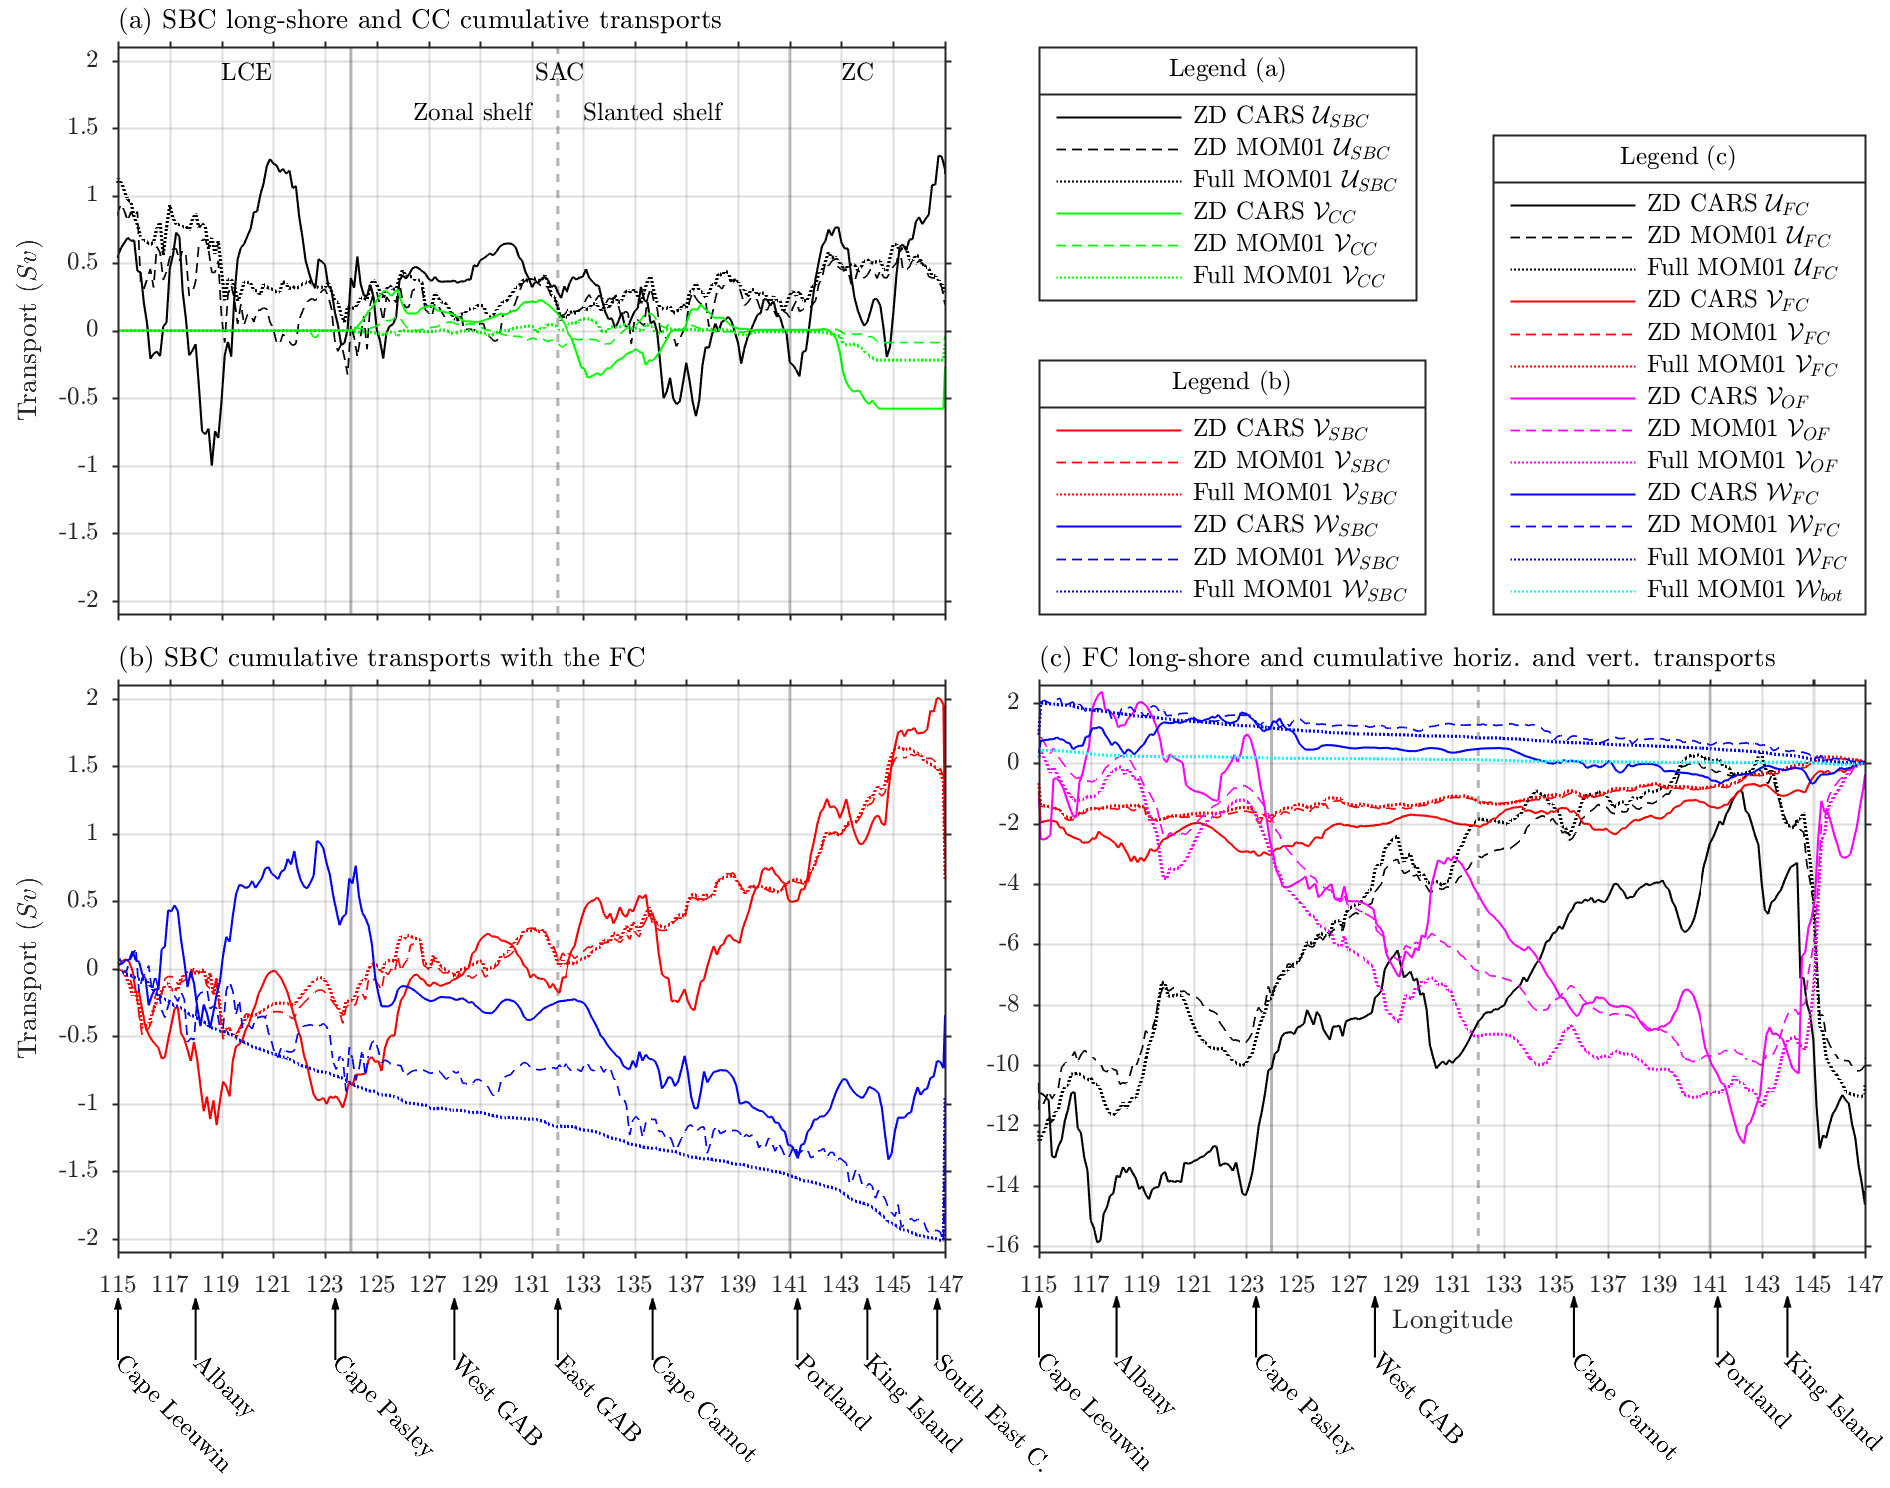
\includegraphics
[width=\textwidth, height=0.89\textheight, keepaspectratio]
{f04_fig1_.png}
\caption{\label{f04_fig1_}%
  Southern Australia Current System transport budget ($Sv$) for (a) the SBC transport (black, positive eastward) and the horizontal cumulative (west to east) cross-boundary transport along $y\sub{CC}$ (green, positive into the SBC), (b) the SBC cumulative (west to east) cross-boundary transport exchanged with the FC horizontally across $y\sub{int}$ (red, positive into the SBC) and vertically across $z\sub{int}$ (blue, positive into the SBC), (c) the FC transport (black, positive eastward), cumulative (east to west) cross-boundary transports with the SBC (red and blue, positive into the FC), and cumulative (east to west) cross-boundary horizontal transport along $y\sub{OF}$ (magenta, positive into the FC). Results are shown for the "Zero Divergence" (ZD, \citeauthor{Furue2017} \citeyear{Furue2017}) adjusted transports in the observations (solid lines) and in the model (dashed lines), and also the actual model transports (thin dotted line). The thin dotted cyan line shows the actual model vertical transport at the bottom of the FC (this is absent in the geostrophic transport). The vertical solid gray lines separate the Leeuwin Current Extension, South Australian Current and Zeehan Current and the vertical dashed grey line separates the region with a zonal shelf to the west from the region with a slanted shelf to the east.}
\end{figure}
%
\begin{figure}[p]
\noindent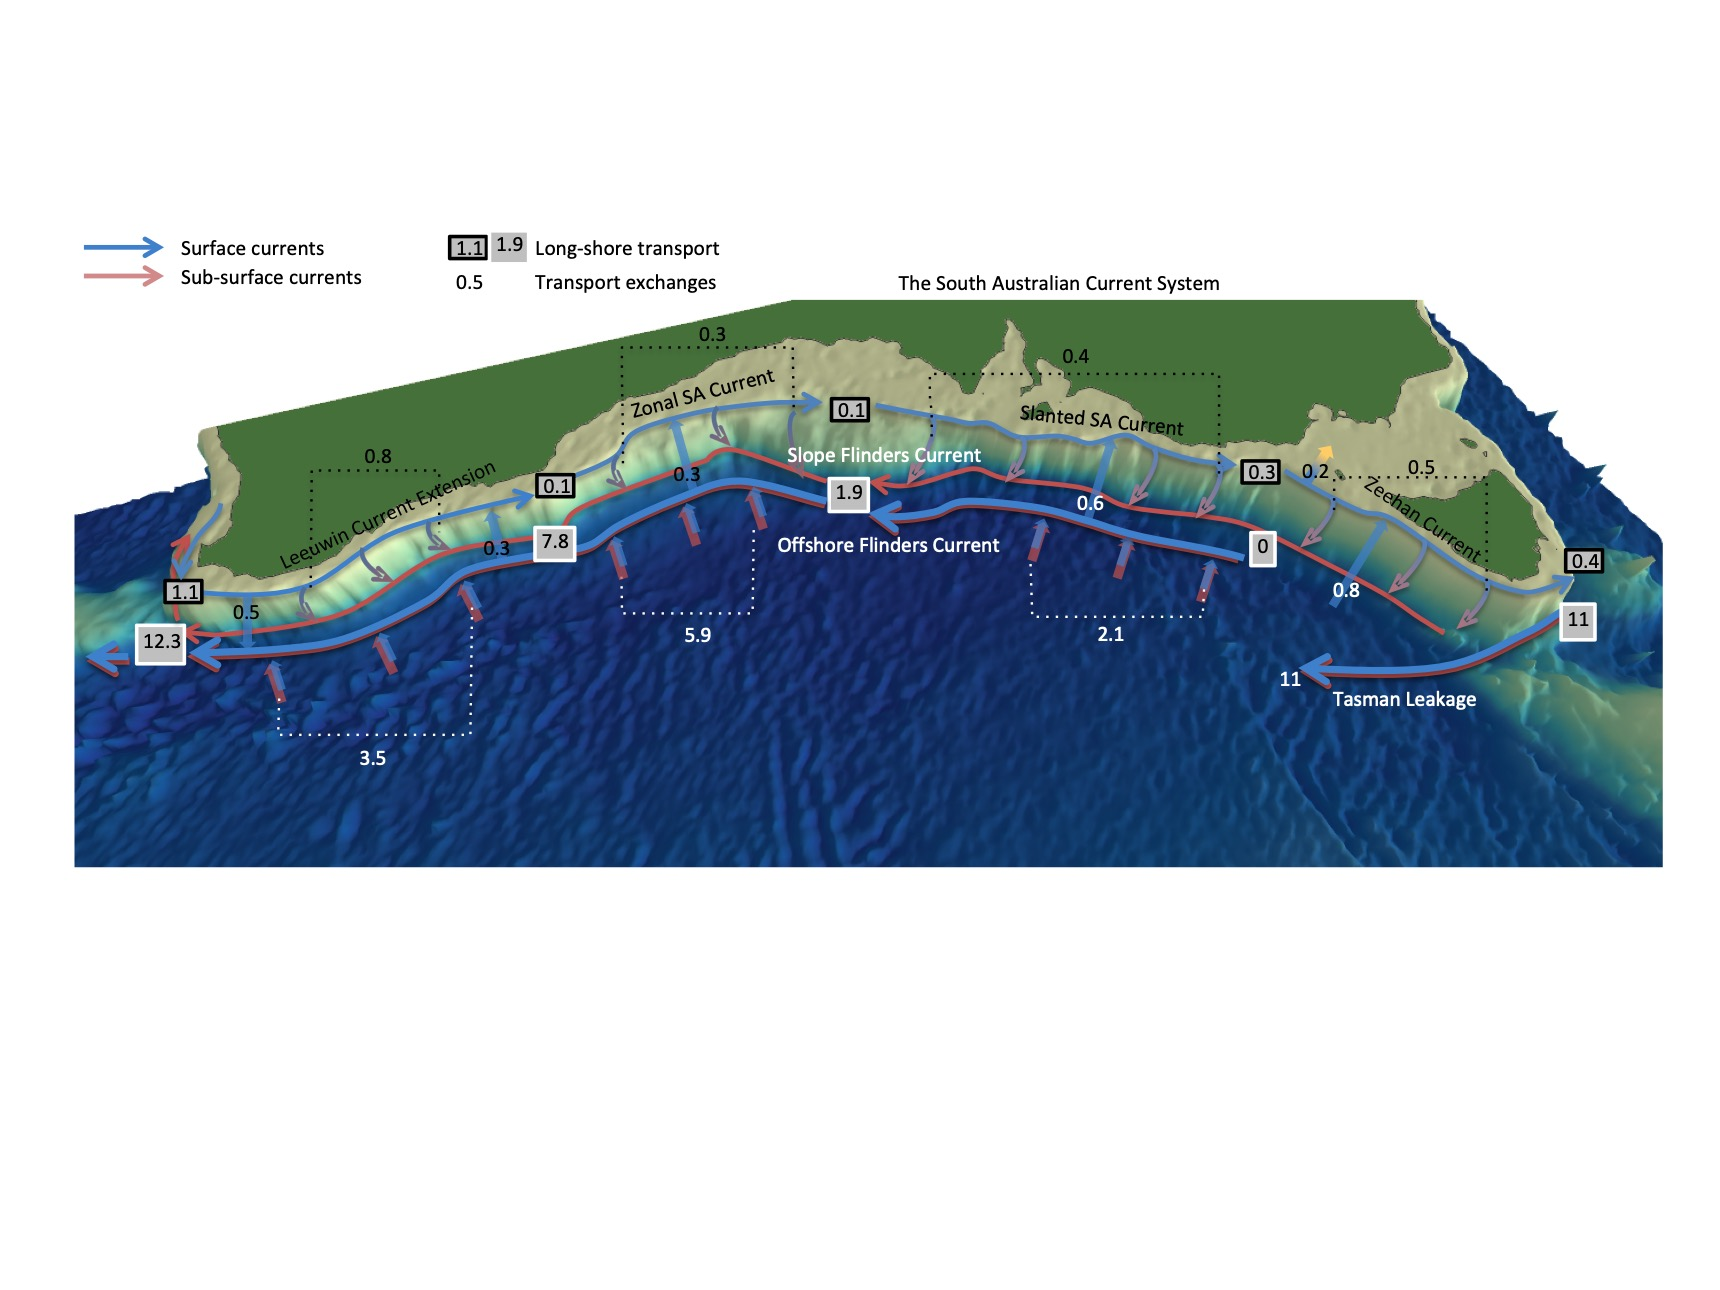
\includegraphics
[width=1\textheight, height=\textwidth, keepaspectratio, angle=90]
{SACS_complex.jpg}
\caption{\label{SACS_complex}%
  Comprehensive Southern Australia Current System transport budget schematics ($Sv$). Transport estimates from MOM01 reported in Section~\ref{Southern Australia Current System Transport Budget} are illustrated here. The SBC transport $\mathcal{U}\sub{SBC}$ (Eq.\,\ref{eq:3}) is shown in the grey box with a black outline. The FC transport $\mathcal{U}\sub{FC}$ (Eq.\,\ref{eq:7}) is shown in the grey box with a white outline. The transport exchanges feeding into the SBC or the FC are shown as plain white or black numbers.}
\end{figure}

The cumulative cross-boundary transport between the coastal current and SBC $\mathcal{V}\sub{CC}$ (Eq.\,\ref{eq:4}, Fig.\,\ref{f04_fig1_}a green lines) in CARS generally exhibits a net inflow into the SBC along the zonal shelf west of \ang{132}E and a net outflow from the SBC along the slanted shelf east of \ang{132}E. These exchanges in the Great Australian Bight and Gulf regions are much weaker in MOM01 with a weak net inflow up to $\mathcal{V}\sub{CC} =$ +\SI{0.1}{Sv}. Since the Bight and Gulfs region
is land-locked, this net transport returns to zero at Cape Jaffa (\ang{139}E)
 and hence this pair of inflow and outflow represents a mean counter-clockwise circulation over the shelf within the Bight and Gulfs.
Over Bass Strait,
there is a net outflow from the SBC of \SI{0.2}{Sv} (Fig.\,\ref{SACS_complex}) in MOM01,
which is half that in CARS\@.

The cumulative cross-boundary transport between the SBC and the FC are presented in Fig.\,\ref{f04_fig1_}b. As seen in the SBC transport, the Leeuwin Current Extension is a region of large difference
between CARS and MOM01,
which is reflected in both the horizontal exchanges with the FC along the SBC south boundary $\mathcal{V}\sub{SBC}$ (Eq.\,\ref{eq:5}, Fig.\,\ref{f04_fig1_}b red lines) and the vertical exchanges with the FC along the SBC bottom boundary $\mathcal{W}\sub{SBC}$ (Eq.\,\ref{eq:6}, Fig.\,\ref{f04_fig1_}b blue lines).
Further east, the downstream trends in the horizontal and vertical exchanges agree reasonably well between CARS and MOM01.
In MOM01, on average the Leeuwin Current Extension loses water horizontally to the FC as the cumulative horizontal transport is negative in the entire Leeuwin Current Extension region. Specifically, the Leeuwin Current Extension loses $\mathcal{V}\sub{SBC} = \SI{-0.5}{Sv}$ up to \ang{119}E near Albany (Fig.\,\ref{SACS_complex}), which indicates
that the Leeuwin Current partly outflows horizontally into the offshore FC as it turns around the south-west corner of Australia to become the Leeuwin Current Extension\@. East of Albany, the opposite happens where the upper offshore FC generally feeds horizontally into the SBC\@. In Fig.\,\ref{SACS_complex} we report the horizontal inflows from the FC into each of the SBC. The total horizontal inflow into the SBC from Cape Leeuwin to South East Cape is +\SI{1.5}{Sv}.

The model vertical exchanges between the SBC and the FC reveal a persistent downwelling out of the SBC that increases steadily from west to east \@. To this downwelling, the Leeuwin Current Extension contributes $\mathcal{W}\sub{SBC} =$ \SI{-0.8}{Sv}, the South Australian Current \SI{-0.7}{Sv} and the Zeehan Current \SI{-0.5}{Sv} (Fig.\,\ref{SACS_complex}). This provides a total downwelling of \SI{-2}{Sv} out of the SBC between Cape Leeuwin and South East Cape (Fig.\,\ref{Slide1}).
Eighty percent of the decrease in the Leeuwin Current Extension's transport from
$\mathcal{U}\sub{SBC} = \num{1.1}$ to \SI{0.1}{Sv} is
due to the downwelling.
The zonal South Australian Current's steady transport of \SI{0.1}{Sv} is maintained by compensating lateral inflows that balance the downwelling in this region. The weak increase
in the slanted South Australian Current's transport and the Zeehan Current's transport is essentially due to an increase in lateral inflows.

To summarise, as the Leeuwin Current Extension flows around the southwest corner of Australia, it loses most of its transport due to downwelling
 and lateral offshore flow.
Then the downwelling is reduced and the western South Australian Current flows along the zonal shelf break without much systematic change in its transport.
As the South Australian Current flows over the slanted shelf break, it receives progressively increasing lateral inflows which are partly overturned by weakly increasing downwelling flows, resulting in a stronger slanted South Australian Current\@.
The Zeehan Current grows
in a similar way,
where the lateral inflow is
strong enough to overcome the losses to the downwelling and a lateral outflow into
Bass Strait. Overall, the SBC transport decreases from $\mathcal{U}\sub{SBC} = \SI{1.1}{Sv}$
at Cape Leeuwin to \SI{0.4}{Sv} at South East Cape is due to a $\mathcal{V}\sub{SBC} = +\SI{1.5}{Sv}$ lateral inflow from the FC minus
a $\mathcal{W}\sub{SBC} = \SI{-2}{Sv}$ downwelling 
back into the FC and a weak lateral $\mathcal{V}\sub{CC} = \SI{-0.2}{Sv}$ shallow loss into Bass Strait.

\subsubsection{FC budget}\label{FC budget}
The FC and cross-boundary cumulative transports are presented in Fig.\,\ref{f04_fig1_}c.
The transport $\mathcal{U}\sub{FC}$ (Eq.\,\ref{eq:7}, Fig.\,\ref{f04_fig1_}c black lines) displays large variations in CARS
as for the SBC\@.
Here the FC is generally stronger in CARS than in MOM01, a difference we noted earlier in the velocity maps (Fig.\,\ref{f03_fig1_}), with a westward transport in the observations up to \SI{6}{Sv} stronger.
In CARS, $\mathcal{U}\sub{FC}$ suddenly becomes
weaker between \ang{117} and \ang{116}E
because of the meridional spreading of the FC noted earlier (Fig.\,\ref{f03_fig1_}a,b).
Otherwise the spatial trends between CARS
and MOM01 are similar.
Both in CARS and MOM01,
the transport undergoes
a sudden loss in westward transport
because of the Tasman Leakage
(see also Fig.\,\ref{f03_fig1_}).
In the model, it varies from $\mathcal{U}\sub{FC} = \SI{-11}{Sv}$
at South East Cape to around zero near Portland (a negative transport is westward). The FC then intensifies along the slanted coast to reach \SI{-1.8}{Sv} at the eastern Great Australian Bight; and along the zonal coast to reach \SI{-7.7}{Sv} at Cape Pasley and \SI{-12.3}{Sv} at Cape Leeuwin (Fig.\,\ref{SACS_complex}). In contrast to the SBC,
the FC thus intensifies systematically as it flows westward.

The exchanges between the FC and the SBC are relatively insignificant in determining this increase in the FC transport as the main contributors to the FC strengthening are the
onshore flows
across the FC's southern boundary (Eq.\,\ref{eq:8}).
The spatial structure of the change
in $\mathcal{U}\sub{FC}$ therefore mirrors
that of $\mathcal{V}\sub{OF}$ (Fig.\,\ref{f04_fig1_}c).

Between South East Cape and \ang{143}E, there is a large outflow of \SI{-11}{Sv},
which is the Tasman Leakage.
From South East Cape to Portland (the Zeehan Current region), the Tasman Leakage loss, the exchanges between the SBC and the FC, and small inputs by onshore flows, result in a zero FC transport at Portland.
In what follows, we describe how $\mathcal{U}\sub{FC}$ changes
in relation to $\mathcal{V}\sub{OF}$, ignoring exchanges with the SBC\@.
%
Between Portland and the eastern Great Australian Bight (the slanted South Australian Current region), the onshore flows provide +\SI{2.1}{Sv} to the FC producing a \SI{-1.9}{Sv} FC transport.
Along the zonal coast, between the eastern Bight
and Cape Pasley (the zonal South Australian Current region), the onshore flows provide a large +\SI{5.9}{Sv} input that
accelerates the FC to \SI{-7.8}{Sv}. Finally, between Cape Pasley and Cape Leeuwin (the Leeuwin Current Extension region), the onshore flows provide a +\SI{3.5}{Sv} input further accelerating the FC to \SI{-12.3}{Sv} (Fig.\,\ref{SACS_complex}).

As an aside, we note that we calculated the accumulated vertical transport along the FC's bottom boundary across $z\sub{ref}$ (Fig.\,\ref{f04_fig1_}c cyan lines and Fig.\,\ref{f02_fig1_}i--p cyan lines).
In our geostrophic calculation, vertical velocity is adjusted to vanish at $z\sub{ref}$.
In the actual velocity field of MOM01, there is a total
upward transport across the \SI{2000}{\meter} depth level of about +\SI{0.25}{Sv}
between South East Cape and Cape Leeuwin, which is very small compared to the FC's large westward transport.
This demonstrates that our choice $z\sub{ref} = \SI{2000}{m}$
was suitable.

In summary, the annual-mean FC is nearly absent off the western Tasmanian shelf and Bass Strait as the Tasman Leakage carries
most
of the westward flow off South East Cape into the South Australian Basin. Along the slanted shelf the FC is weak as the onshore flows feeding into the current are small. When the shelf becomes zonal,
the onshore flows are much stronger, providing a large source water for the FC\@.
Overall, after the Tasman Leakage loss (\SI{-11}{Sv}),
the FC transport increases from zero to $\mathcal{U}\sub{FC} = \SI{-12.3}{Sv}$
at Cape Leeuwin due to a net +\SI{11.8}{Sv} gain from the onshore flows (Fig.\,\ref{Slide1}). Out of this net inflow, 2.5\% occurs west of Tasmania, 17.8\% along the slanted shelf, 50\% in the zonal Great Australian Bight region and 29.7\% in the zonal shelf region from Cape Carnot to Cape Leeuwin. Therefore, nearly 80\% of the onshore flow contribution to the FC increase occurs along the zonal shelf. Another \SI{+0.5}{Sv} net gain from the SBC comes from downwelling flows which only contribute to about 4.1\% of the FC's total increase. 

\subsection{SBC and FC coupling}\label{SBC and FC coupling}
The Southern Australian Current System transport budget revealed that a large part of the onshore flow into the FC is directly converted into increasing westward transport from close to zero along western Tasmania to \SI{12.3}{Sv} near the western side of Australia.

Further inshore, there is a coupling between the SBC and offshore FC which provides a lateral source water for the SBC\@. We examine maps of Ekman drift in Fig.\,\ref{f18_fig1_} to provide a mechanism for such lateral inflow into the SBC\@. We find that the annual-mean Ekman drift in ERA-Interim (which was used with the CARS geostrophic velocities to calculate the transport in CARS, Fig.\,\ref{f18_fig1_}a) is slightly stronger than the Ekman drift in CORE2-NYF (which was used to force MOM01, Fig.\,\ref{f18_fig1_}b). The Ekman drift is generally pointing northward, hence onshore everywhere except in the Great Australian Bight and southeast in front of the Gulfs where it decreases and turns westward. The onshore Ekman drift provides a coupling mechanism between the offshore FC and SBC, explaining the lateral inflow from the offshore FC into the SBC.
%
\begin{figure}[htp]
\noindent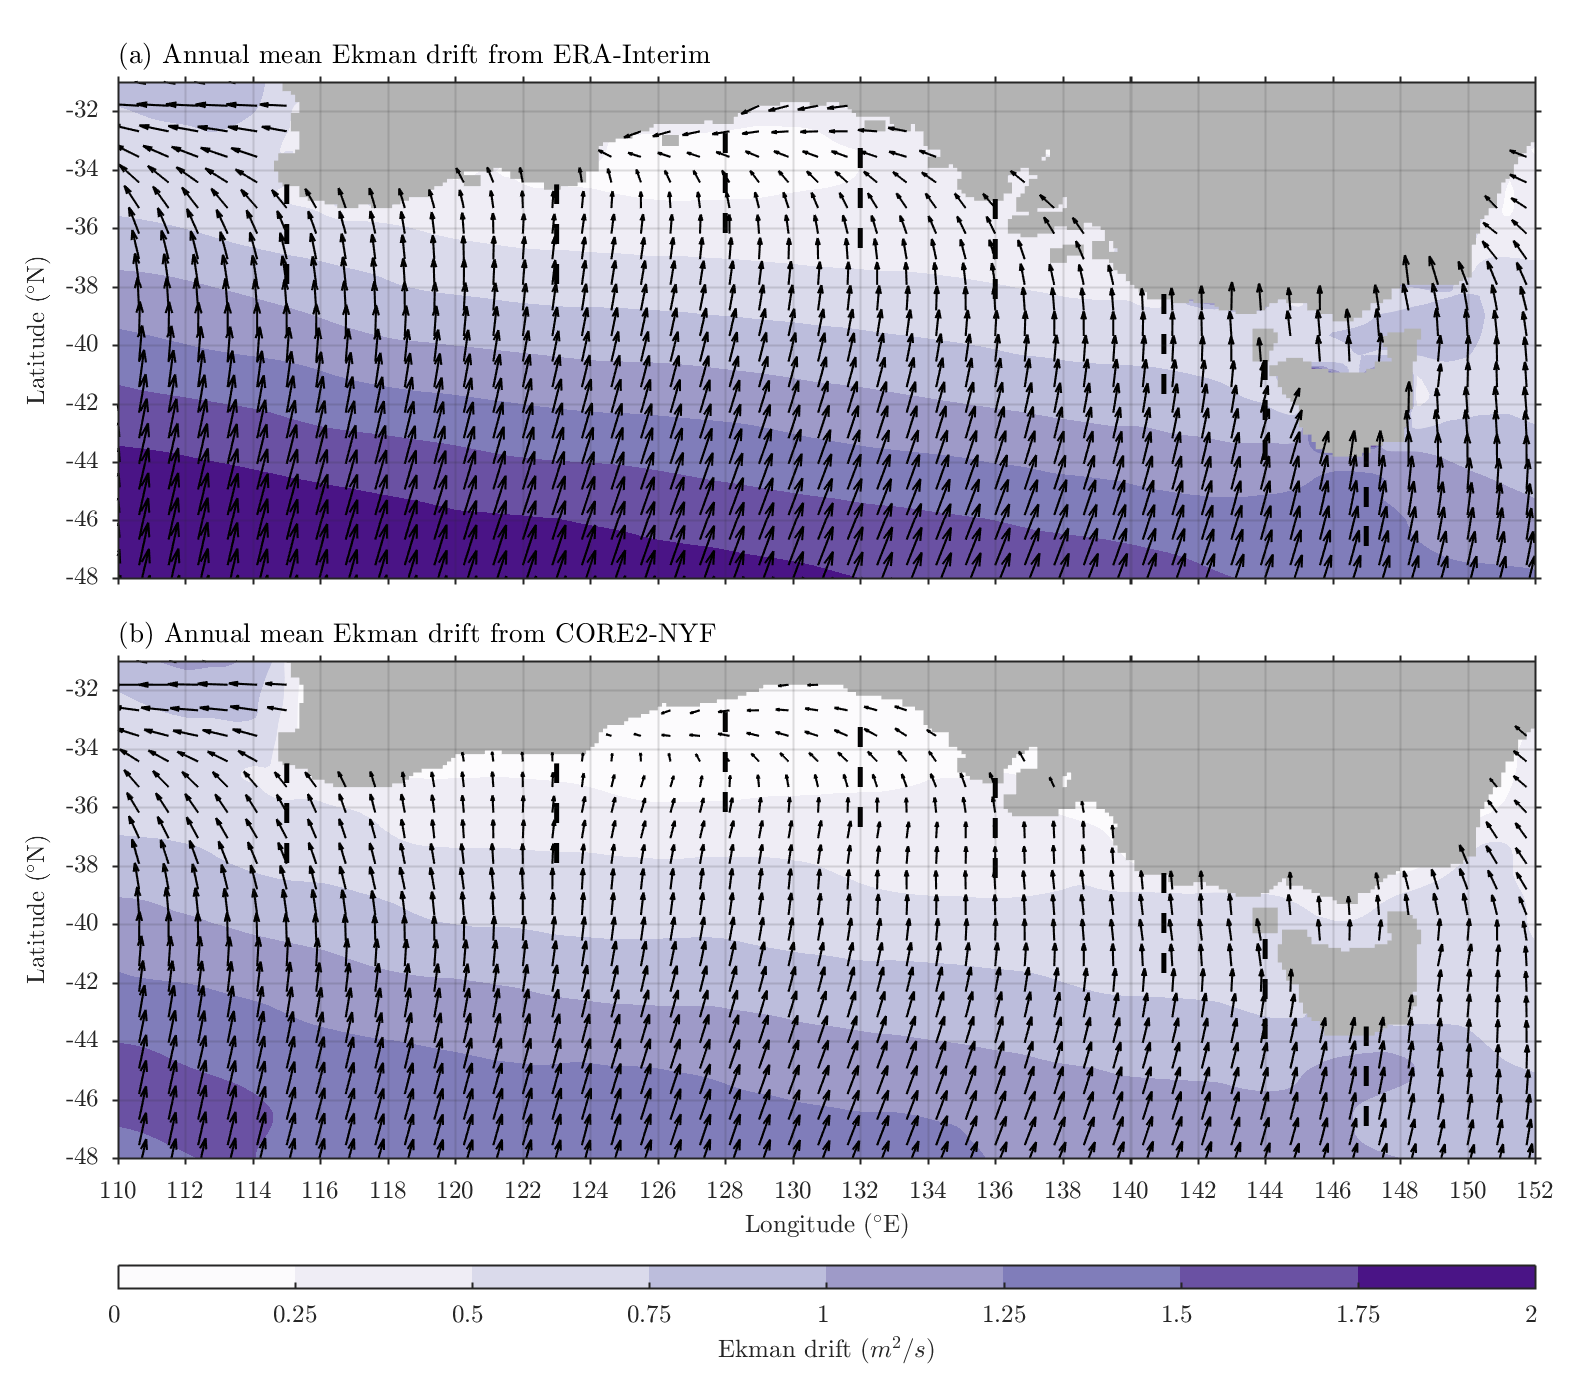
\includegraphics
[width=\textwidth, height=0.89\textheight, keepaspectratio]
{f18_fig1_.png}
\caption{\label{f18_fig1_}%
    Long-term mean Ekman drift (\si{\square\meter\per\second}) estimated from (a) ERA-Interim winds and (b) CORE2-NYF winds (see Section~\ref{Datasets}). The magnitude of the Ekman drift is indicated by the shading. To illustrate weaker flows better, arrow lengths are proportional to the square root of the vector amplitudes.}
\end{figure}

The transport budget also revealed a coupling between the SBC and the slope FC where the aforementioned Ekman drift is downwelled into the slope FC\@. We examine maps of vertical flows along $z\sub{int}$ in MOM01 in Fig.\,\ref{f16_fig1_} to examine the spatial variability of the annual-mean downwellings along the coast. We note that we do not show the vertical velocities produced by the Zero-Divergence adjustment, neither in this Figure nor in Fig.\,\ref{f07_fig1_}. This is because the geostrophic calculation (before and after the Zero-Divergence adjustment) produces a noisy vertical-velocity field above complex bottom topography (evident in Fig.\,\ref{f04_fig1_}b,c in local reversal in accumulated upwellings/downwellings). Thus, these fields are useful only when integrated over a long distance as in our cumulative transport calculations. For example, the longshore integration of vertical velocities at the base of the SBC (Eq. \ref{eq:6}) reveals the vertical velocity that compensates the SBC flow above it.
%
\begin{figure}[ht]
\noindent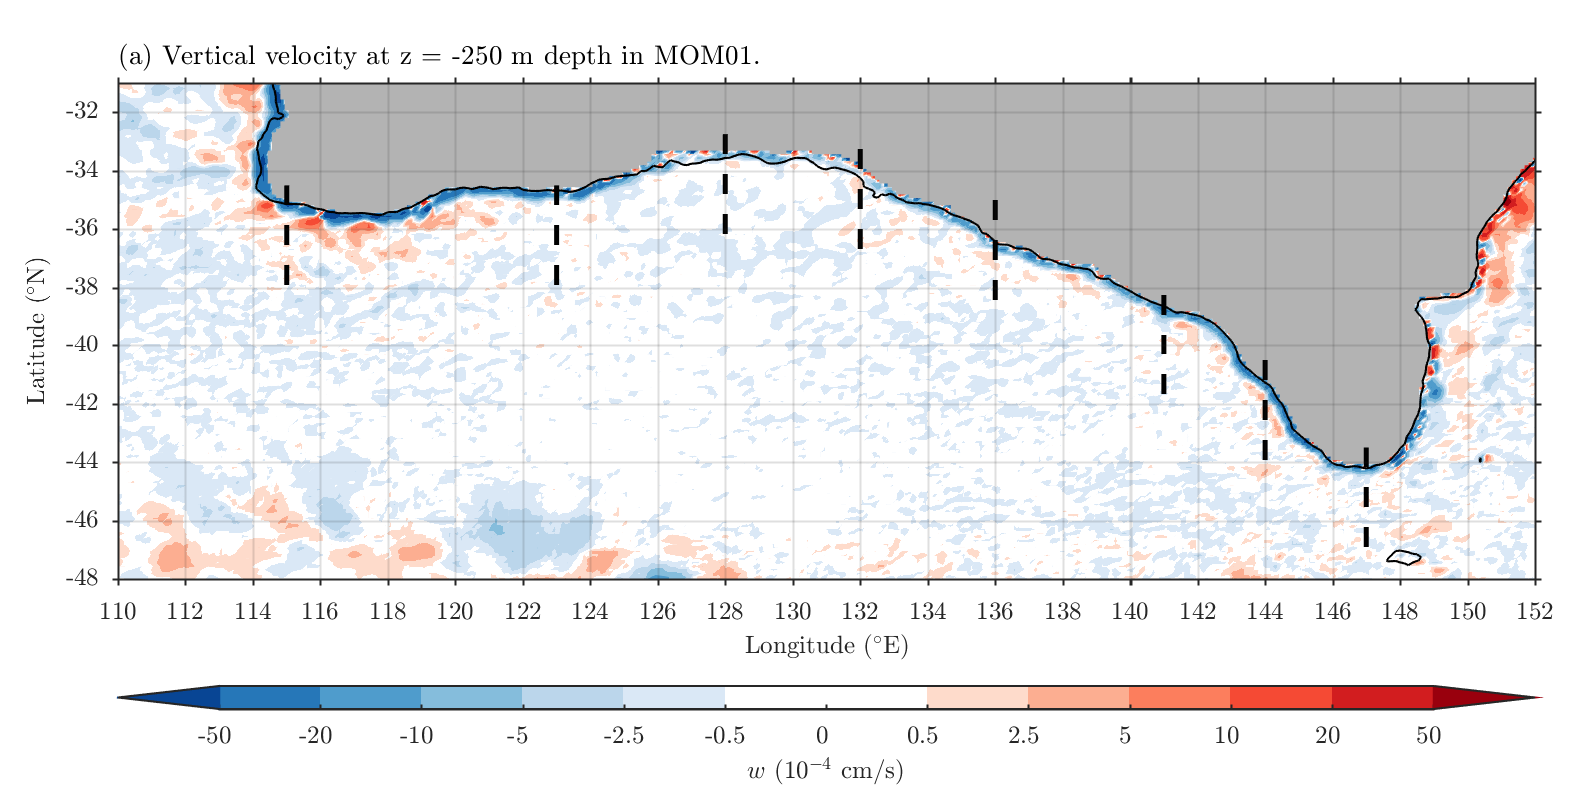
\includegraphics
[width=\textwidth, height=0.89\textheight, keepaspectratio]
{f16_fig1_.png}
\caption{\label{f16_fig1_}%
    Long-term mean full model vertical velocity field at $z\sub{int} = -250$ \si{\meter} in $10^{-4}$ \si{\centi\meter\per\second} (with nonlinear shading levels) in MOM01. The thin black line shows the 1000 \si{\meter} isobath. The grey region is where $z > -250 m$.}
\end{figure}

The vertical flows along the upper slope at \SI{-250}{\meter} are downwelling throughout the southern Australian shelves. The downwelling is strong where the slope is steep particularly outside the Great Australian Bight region. In the Bight, the slope is less steep and the downwelling is weaker. The primarily onshore direction of the Ekman drift is consistent with the downwelling found all along the coast. The downwelling is most pronounced in the Leeuwin Current Extension and Zeehan Current regions, where the onshore Ekman drift is strongest (Fig.\,\ref{f18_fig1_}). In the Bight and Gulf regions the Ekman drift curls anti-clockwise resulting in weak downwelling, which is further reduced in the Bight where the slope is less steep.

Finally, there is also an inverse seasonal relationship between the SBC and the FC which we briefly discuss here. Fig.\,\ref{f19_fig1_} shows the summer and autumn states in MOM01 for the SBC transport ($\mathcal{U}\sub{SBC}$, Fig.\,\ref{f19_fig1_}a) and the FC transport ($\mathcal{U}\sub{FC}$, Fig.\,\ref{f19_fig1_}b). We show the summer and the autumn states only as they exhibit the strongest deviation from the annual-mean. Winter and spring states are much closer to the annual-mean (not shown). \citet{Oke2018} also found that the SBC are strongest in autumn, decrease in winter and spring and are weakest in summer. 
%
\begin{figure}[p]
\noindent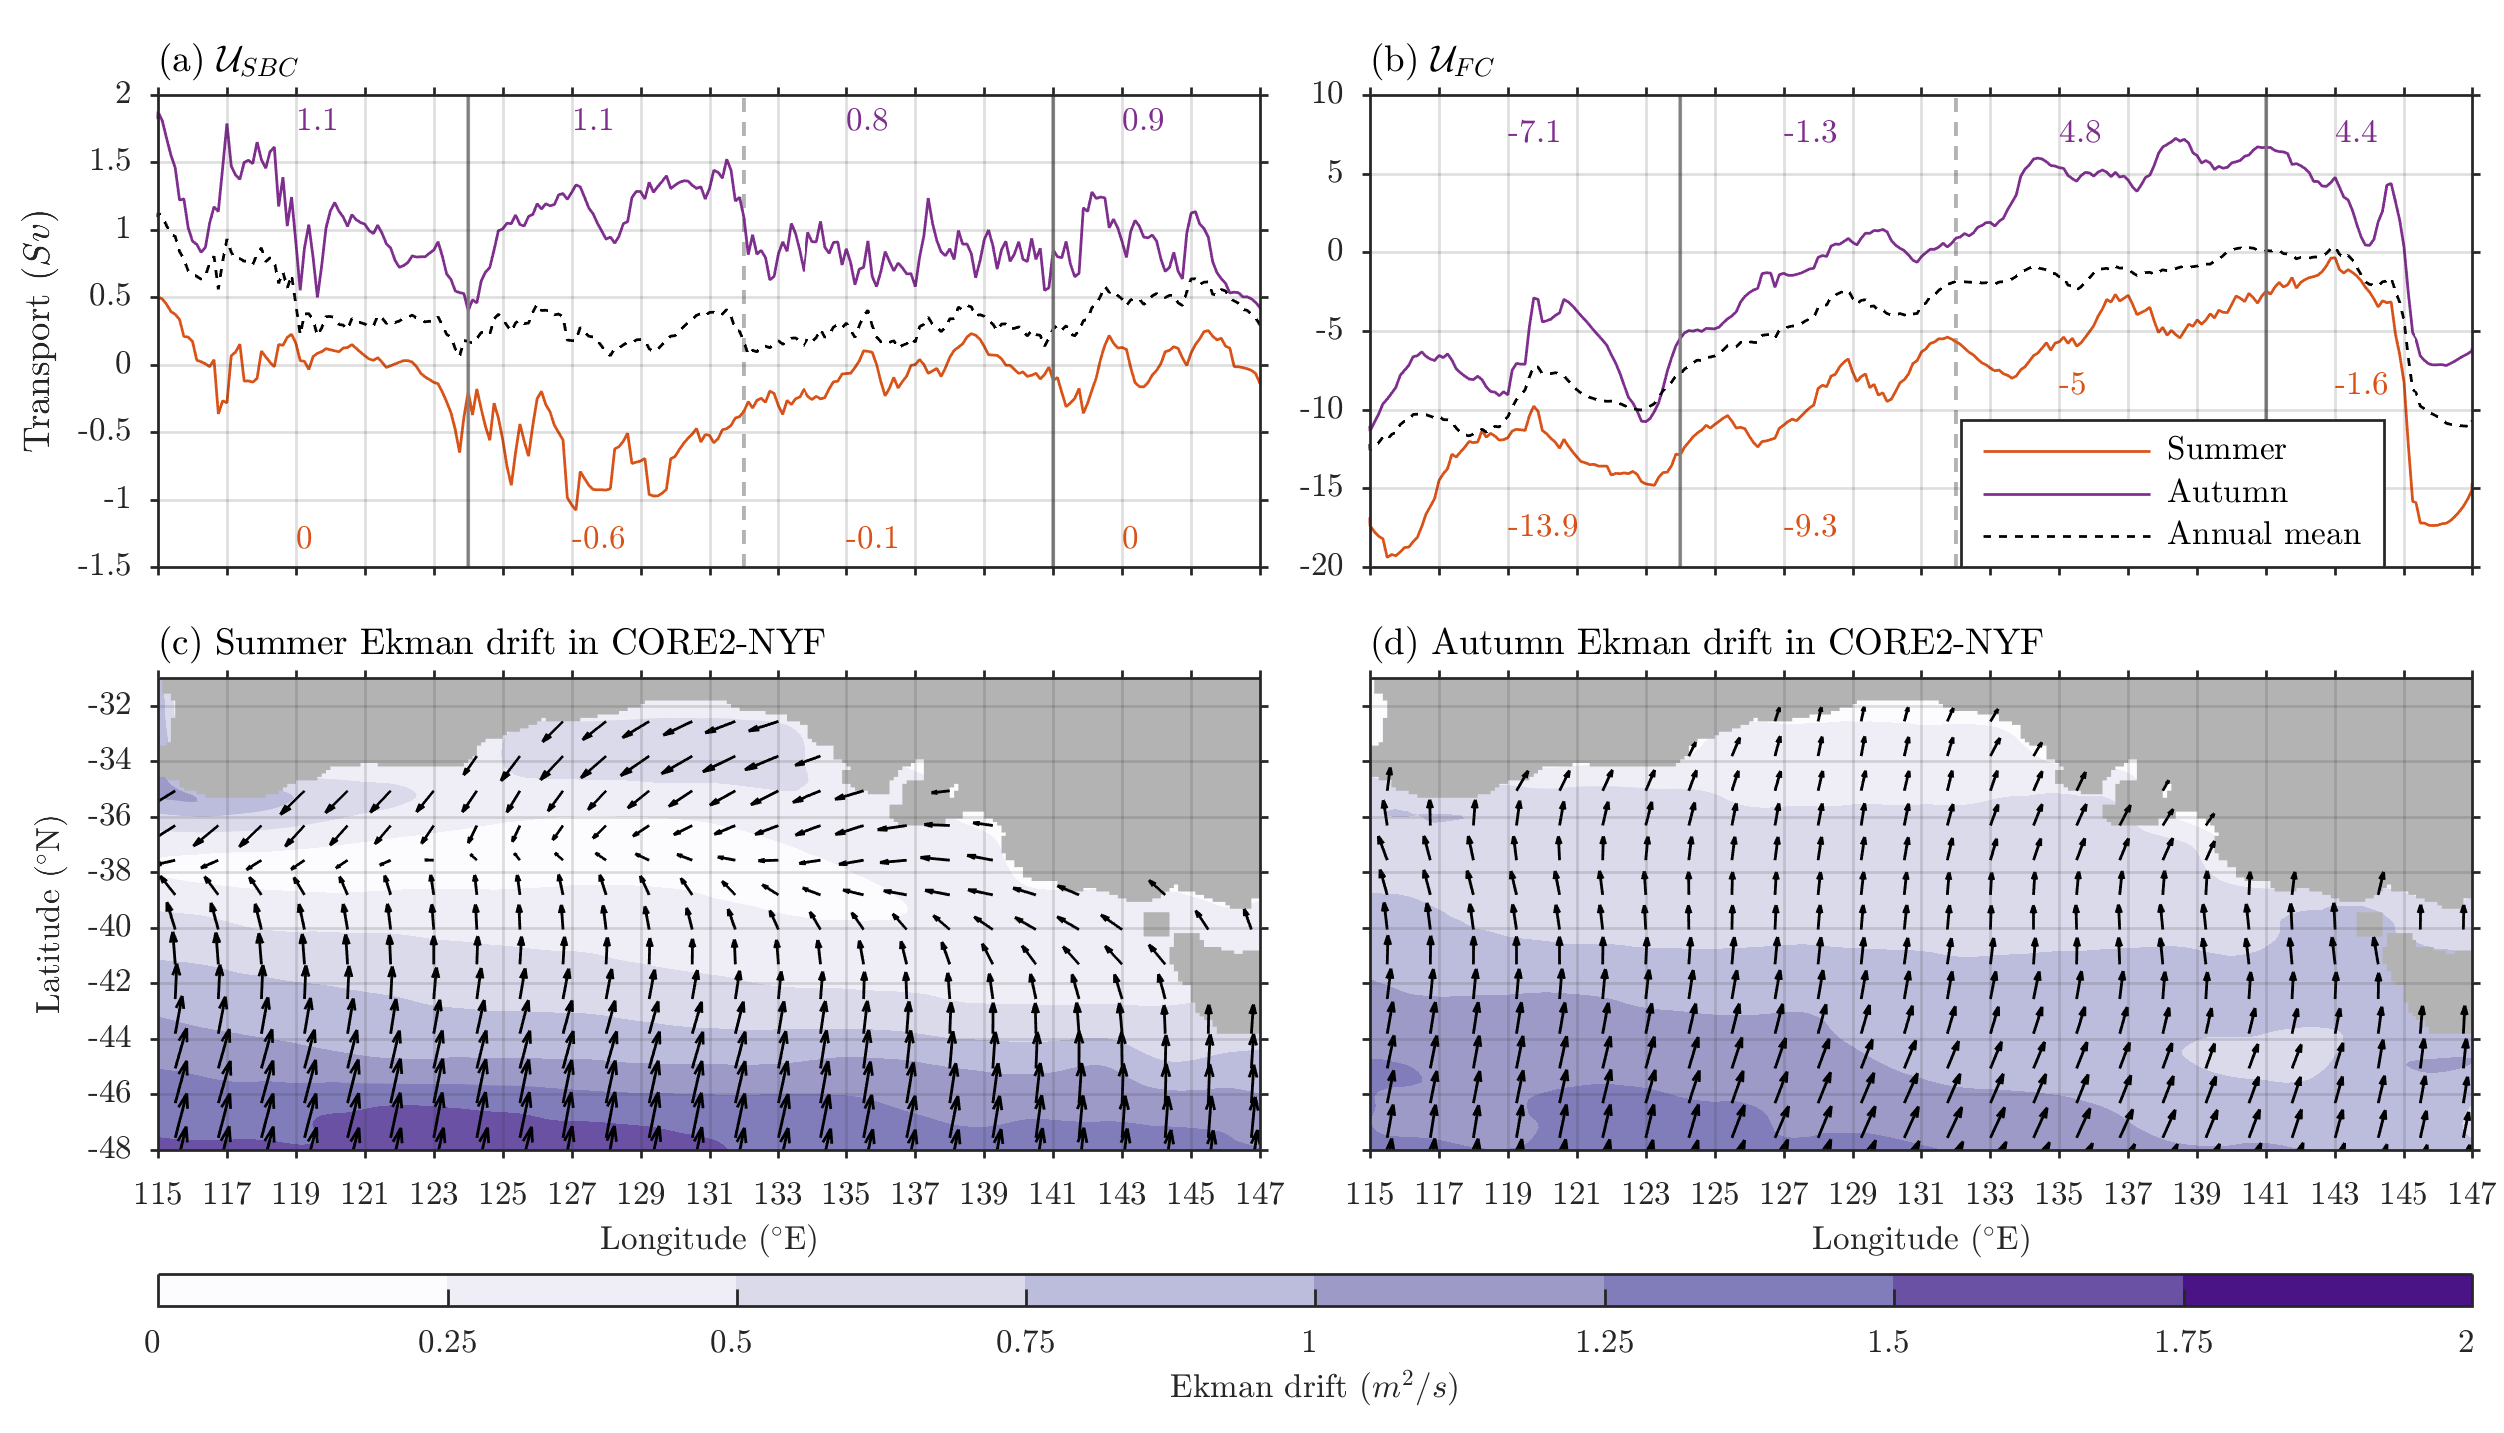
\includegraphics
[width=\textwidth, height=0.89\textheight, keepaspectratio]
{f19_fig1_.png}
\caption{\label{f19_fig1_}%
    Summer mean (orange lines), autumn mean (purple lines), annual-mean (black dashed lines) in MOM01 for (a) the SBC transport ($\mathcal{U}\sub{SBC}$, positive eastward) and (b) the FC transport ($\mathcal{U}\sub{FC}$, positive eastward); and Ekman drift derived from CORE2-NYF winds in (c) summer and (d) autumn. In (a) and (b), the vertical solid gray lines separate the Leeuwin Current Extension, South Australian Current and Zeehan Current and the vertical dashed grey line separates the region with a zonal shelf to the west from the region with a slanted shelf to the east. The coloured numbers in (a) and (b) show, from left to right, the mean transport in the Leeuwin Current Extension region, the zonal South Australian Current region, the slanted South Australian Current region and the Zeehan Current region in summer (orange) and in autumn (purple). In (c) and (d), the magnitude of the Ekman drift is indicated by the shading whereas arrow lengths are proportional to the square root of the vector amplitudes.}
\end{figure}

In summer, the SBC are weakest and reversed in many places along the coast, particularly in the zonal South Australian Current region (Fig.\,\ref{f19_fig1_}a). On average, the Leeuwin Current Extension, the slanted South Australian Current and the Zeehan Current carry very little eastward transport, and the zonal South Australian Current is strongly westward at \SI{0.6}{Sv} on average with a maximum westward transport reaching \SI{1}{Sv}. The zonal South Australian Current exhibits the largest seasonal changes in transport. In summer, the weak SBC can be explained by the mostly offshore direction of the Ekman drift along the coast, particularly in the Great Australian Bight (Fig.\,\ref{f19_fig1_}c). The strengthening of the SBC occurs in autumn when the westerlies start strengthening and shifting north as shown by the strong basin-wide onshore Ekman drift (Fig.\,\ref{f19_fig1_}d). Indeed, the SBC are strongest in autumn with an average eastward transport between 0.8 and 1.1 Sv and a maximum eastward transport up to 1.75 Sv (Fig.\,\ref{f19_fig1_}a).

The FC also displays a strong seasonal variability (Fig.\,\ref{f19_fig1_}b). In summer, the FC is strongest along both the slanted and the zonal shelf. Near the south-west corner of Australia, the FC carries on average \SI{13.9}{Sv} westward, with maximum transport around \SI{19}{Sv}. In autumn, the FC is weakest, eastward along the slanted shelf (average eastward transport up to \SI{4.8}{Sv}), and westward along the zonal shelf with an average westward transport of \SI{7.1}{Sv} off south-western Australia. The SBC and the FC therefore have a seasonally opposed strengthening--weakening cycle and the SBC--offshore-FC pairing is affected by the Ekman drift's seasonality. For instance the summer transport is dominated by the strongly westward FC with little to no eastward transport from the SBC\@. In autumn, the transport from the SBC is strongly eastward whereas the slanted FC is reversed. We expect the SBC--slope-FC pairing via downwelling and onshore flows feeding into the FC to also exhibit a strong seasonality, which will be examined in a future study.

\section{Summary and Closing Discussion}\label{Summary}
We investigated the structure, transport budget and coupling of currents in the Southern Australia Current System and have provided a comprehensive
description
of the circulation along the southern shelves of Australia and the South Australian Basin. The Southern Australia Current System contains the eastward Shelf Break Currents (SBC),
which include the consecutive Leeuwin Current Extension, South Australian Current and Zeehan Current from west to east and the counter-flowing westward Flinders Current (FC) both offshore and underneath the SBC\@.
We defined the zonal sector between Cape Leeuwin (\ang{115}E) and the eastern Great Australian Bight (\ang{132}E) where the continental margin is approximately zonal 
and the slanted sector between the eastern Bight and South East Cape south of Tasmania (\ang{147}E),
where the margin is slanted. We used CARS, a long-term average of hydrographic observations gridded at a 1/\ang{8} resolution
and MOM01, a 7-year
subset of a long-term OGCM simulation
at a 1/\ang{10} resolution
forced by a repeated climatological annual cycle of
atmospheric conditions.
We derived mass-conserving flows from temperature and salinity fields and defined the boundaries of the SBC and the FC to produce a closed transport budget. The purpose of this work was to
synthesize past observational and modelling results into a comprehensive picture
of the Southern Australia Current System. The agreement we find between the observations and the model provide confidence that the methodology used here and in \citepos{Furue2017} can be useful to other boundary circulations. This paper also aims to serve as a framework for a future study on the seasonality and mechanisms of the system. 

\subsection{Southern Australia Current System structure}
In general, the annual-mean SBC agreed well between CARS and MOM01 (Fig.\,\ref{f02_fig1_}~and~\ref{f03_fig1_}). The SBC are confined to
 the upper \SI{250}{m} with a maximum speed of \SI{20}{cm.s^{-1}}.
The SBC are fairly continuous all along the shelf break
(Fig.\,\ref{f03_fig1_}a,b~and~\ref{f04_fig1_}a)
with a weakening Leeuwin Current Extension between Cape Leeuwin and Cape Carnot (\ang{124}E); a stable zonal South Australian Current between Cape Carnot and the eastern Great Australian Bight; a strengthening slanted South Australian Current between the eastern Bight and Portland (\ang{141}E) and an also strengthening Zeehan Current between Portland and South East Cape.

In general, the FC speed in CARS was in good agreement with individual observational records, and was stronger than in MOM01.
The FC has a dual structure with a slope FC core located along the continental slope around \SI{600}{\meter} depth, which is an undercurrent for the SBC, and an offshore FC core 
which is weak and patchy or even reverses along the slanted coast but becomes stronger and better defined in the zonal sector (Fig.\,\ref{f02_fig1_}~and~\ref{f03_fig1_}).

There is a net downwelling
from the lower and seaward portion of the SBC into the slope FC
in regions with a steep continental slope (Fig.\,\ref{f07_fig1_}).
In one cross-shore section where the slope was significantly gentler, the slope FC was absent and the SBC bottom flows were actually weakly upwelling. Generally, along the zonal shelf, the downwelling is weak (except off Cape Leeuwin, greater than \SI{-50 e-4}{\centi\meter\per\second}) and in the upper \SI{600}{\meter}. Along the slanted shelf, the downwelling is strong (greater than \SI{-20 e-4}{\centi\meter\per\second}) and in the upper \SI{1000}{\meter}. These findings suggest that the downwelling from the SBC is important in maintaining the slope FC which emerges along the slanted slope where the downwelling is strongest.

There is an eastward jet to the south of the offshore FC, which is particularly well defined in the zonal sector (Fig.\,\ref{f03_fig1_}).
This newly reported jet extends
to \SI{2000}{\meter} in the zonal sector (Fig.\,\ref{f02_fig1_}) and is weaker and confined to the upper \SI{250}{\meter} in the slanted sector,
where it bends south-eastwards along and into the slanted FC\@.
This jet is probably an expression of the southern arm
of the Albany High (see Introduction Section~\ref{The Deep-Ocean Circulation}),
a persistent regional anti-clockwise gyre centred offshore of Albany (\ang{118}E) with the zonal FC as the northern westward arm and the eastward jet as the southern eastward arm.

\subsection{Southern Australia Current System transport budget}
The transport budget qualifies and quantifies the spatial evolution of the annual-mean SBC and FC and the results are
schematically summarized in
Fig.\,\ref{Slide1}.
%
\begin{figure}[p]
\centering%
\includegraphics%
[width=1\textheight, height=\textwidth, keepaspectratio, angle=90]
{Slide1.jpg}
\caption{\label{Slide1}%
  Southern Australia Current System summary transport budget schematics. Long-shore transport for the SBC and FC in grey box with orange outline and white outline, respectively. Integrated vertical and onshore flows transport in dashed outline box. For visibility, white (black) text is overlaid on dark (light) background.}
\end{figure}

The Leeuwin Current turns around the southwest corner of Australia
to become, or feed into, the Leeuwin Current Extension\@.
Its initial transport is \SI{1.1}{Sv} eastward
but it
loses a part of its transport to downwelling
and, to a lesser extent, to lateral offshore flows near Cape Leeuwin. The Leeuwin Current Extension eventually carries \SI{0.1}{Sv} as it approaches the Great Australian Bight.
The western South Australian Current flows along the zonal shelf break
without substantial changes in transport.
As the South Australian Current flows over the slanted shelf break, it receives more lateral inflow than the loss to downwelling and is consequently accelerated to \SI{0.3}{Sv}.
The Zeehan Current grows under the same process to \SI{0.4}{Sv} where lateral inflows are strong enough to overcome both downwelling
and a loss into Bass Strait.
Overall, the SBC transport
decrease from Cape Leeuwin to South East Cape
is due to
a $\mathcal{V}\sub{SBC} = +\SI{1.5}{Sv}$ lateral inflow 
from the FC, which is in turn downwelled as $\mathcal{W}\sub{SBC} = \SI{-2}{Sv}$ that feeds back into the FC and a $\mathcal{V}\sub{CC} = \SI{-0.2}{Sv}$ shallow lateral loss into Bass Strait.

The annual-mean FC is weak or absent
off the western Tasmanian shelf and Bass Strait
as the Tasman Leakage carries
away most of the FC transport (\SI{-11}{Sv})
near South East Cape due westward into the South Australian Basin. The onshore flows along the slanted shelf are weak and result
in only a weak increase to the FC transport (\SI{1.9}{Sv})
in the eastern Great Australian Bight. When the shelf becomes zonal, the onshore flows are much stronger and
accelerate the FC to
\SI{7.8}{Sv} by Cape Carnot
(the western end of the Bight)
and to \SI{12.3}{Sv} by Cape Leeuwin.
Overall, 2.5\% of the net onshore flows occur west of Tasmania, 17.8\% along the slanted shelf, 50\% (\SI{-5.9}{Sv})
in the zonal Great Australian Bight,
and 29.7\% in the zonal shelf region from Cape Carnot to Cape Leeuwin. Therefore, nearly 80\% of the onshore flow contribution to the FC increase occurs along the zonal shelf. Another \SI{+0.5}{Sv} net gain from the SBC comes from
downwelling, which
accounts for only about 4.1\% of the FC's total increase.


\subsection{Closing discussion}\label{Closing discussion}
The continuity of the near-surface shelf break currents extending from Northwest Cape off Western Australia to Southeast Cape off Tasmania has been understood since \citet{Ridgway2004} described them as a 5500 km long boundary current. The two components are the Leeuwin Current System off Western Australia and the collection of currents south of Australia that we here define as the Southern Australia Current System. The volume transport and spatial variability of the Leeuwin Current System was quantified in \citet{Furue2017}. Here, we have quantified the transport and spatial variability of the Southern Australia Current System, consisting of the eastward SBC and the counter-flowing westward FC that has a slope-trapped part forming an undercurrent to the SBC, and a deep-reaching offshore part. 

The dual analysis of observations and model in this study, goes beyond the traditional approach of validating a model based on a range of indices available from observations, and then analyzing spatial and temporal variability using the model alone. We find here that applying identical methods to both model and observations, leads to enhanced confidence in the structure and transport of the Southern Australia Current System.

In this work, we have discovered a coupling between the SBC and slope FC through downwelling, and between the SBC and offshore FC through onshore Ekman drift. The annual-mean Ekman drift is largely onshore along the Southern Australian shelves (Fig.\,\ref{f18_fig1_}). In the Great Australian Bight and in front of the Spencer and St Vincent Gulfs, the Ekman drift curls anti-clockwise resulting in weaker onshore Ekman transport. The onshore Ekman transport is consistent with downwelling flows which are strongest where the shelf is steep, that is everywhere outside of the Great Australian Bight (Fig.\,\ref{f16_fig1_}).

On one hand, the combined effect of the horizontally coupled SBC--offshore-FC pair and vertically coupled SBC--slope-FC pair is a conversion of a widespread northward Ekman drift into downwelling with little impact on the transport of the SBC\@. On the other hand, a large part of the onshore flows into the FC is directly converted into increasing westward transport from close to zero along western Tasmania to \SI{12.3}{Sv} near the western side of Australia. 

The SBC--slope-FC pair bears a striking similarity with the Leeuwin-Current--Leeuwin-Undercurrent (LC--LUC) pair described in \citet{Furue2017}. The LC--LUC pair is driven by the onshore geostrophic flow due to the meridional density gradient in the southeast Indian Ocean, and the SBC--slope-FC pair is driven by the onshore Ekman drift. From the annual-mean perspective, the dynamical balance of both systems could be the same, with strong onshore flows being overturned into an undercurrent.

While this work has focused on the mean structure of the Southern Australia Current System, its temporal variability is of major interest for future work. \citet{Ridgway2015} for example examined the seasonal cycle of the Leeuwin Current System and found that annual pressure signals originating from north of Australia propagate around Australia counter-clockwise, reaching to Tasmania. In the present paper, a brief analysis of the SBC and FC summer and autumn states showed that the SBC--offshore-FC pairing via Ekman drift is significantly modified by the Ekman drift's seasonality. In summer, the Ekman drift is mostly oriented offshore which drives weak SBC that are reversed to westward in some places, particularly in the Great Australian Bight where the zonal South Australian Current flows (Fig.\,\ref{Slide1}). Conversely, the FC dominates the longshore transport as it is at its strongest in summer and transports up to \SI{19}{Sv} westward. In autumn, the Ekman drift is stronger and oriented onshore due to the westerly winds starting to shift north and strengthen in this season. This drives strong SBC with an eastward transport up to \SI{1.75}{Sv} while the FC is at its weakest and reversed along the slanted shelf (Fig.\,\ref{Slide1}). In the Leeuwin Current System, the Leeuwin Current undergoes a seasonal cycle \citep{Ridgway2015} but does not strongly reverse like the zonal South Australian Current does in summer or the slanted FC does in autumn. In the domain of the present study, there is a significant seasonal cycle in winds, which contributes to the seasonal cycle of the SBC and the FC and is likely to contribute to other aspects of the Southern Australia Current System such as the SBC--slope-FC pairing via downwelling and the onshore flows feeding into the FC\@. This will be the focus of a future study. 

Slower timescale variability in this boundary current system is also of interest. For example, \citet{Feng2003} documented the impact of ENSO on the transport variability of the Leeuwin Current System. A prevailing La Ni\~na state was found to be a key contributor to the devastating 2011 marine heat wave off Western Australia \citep{Feng2013}. The impact on the Southern Australia Current System of large-scale climate modes, such as ENSO and the Southern Annular Mode, and their impact on marine climate along the southern Australian coastline have yet to be defined. The consistency between CARS and the MOM01 model in this work suggests that the model is well suited to this task. New observations of this under-sampled boundary current are essential to ground-truth the model results.

\section{Acknowledgment}
This study was supported by the Australian Research Council Discovery Projects (DP130102088) and by the National Science Foundation through Grant OCE-0961716. We thank Jeff Dunn for updating the CARS Aus8 dataset (\url{http://www. marine.csiro.au/atlas/}). ERA-Interim data is publicaly available on \url{https://www.ecmwf.int/en/forecasts/datasets/archive-datasets/reanalysis-datasets/era-interim}. MOM01 data is publicaly available on \url{http://cosima.org.au/index.php/models/access-om2-01-2/}. ED thanks the Consortium for Ocean-Sea Ice Modelling in Australia (COSIMA, \url{http://cosima.org.au}) and the Australian National Computing Infrastructure for making the MOM01 run possible. This work benefited from discussions with Matthew England. ED was supported by the Australian Research Council Centre of Excellence for Climate System Science. HP and NB acknowledge funding from the Australian Government's National Environmental Science Programme. RF was partially supported by the Japan Society for the Promotion of Science through KAKENHI 16K05562.
Funding
  from the ARC Centre of Excellence for Climate Systems Science
  and the University of Tasmania enabled RF to visit the lead author's
  institute.
PS was supported by an Australian Research Council (ARC) DECRA Fellowship DE150100223.

\appendix
\setcounter{figure}{0}
\section{On the definition of longshore transport} \label{Reasoning for defining the SBC transport and the FC transport from their zonal transport}
This appendix discusses the definition of the transport for a longshore current. In the main text, we integrate zonal velocity instead of longshore velocity to define the transport of the SBC or FC (Section\,\ref{Transport budget derivation}) Here we explain why our volume-conserving approach is the best method to use.

\subsection{On using gridboxes to construct the control volume for leak-free calculations}
The central part of this study is to develop a transport budget for the Southern Australia Current System. To do this, it is essential that the currents are captured by control volumes with horizontal and vertical boundaries that fully enclose the currents. Details of this are provided in Section\,\ref{SBC and FC definition}.

Once the control volumes of the currents are defined, we can use conservation of mass to derive the transports of the longshore current by adding all the horizontal and vertical transports across the faces of the control volumes. The faces of our control volumes are set to coincide with faces of the underlying gridboxes. This arrangement enables an exact closure of volume budget except for the tiny truncation error at machine precision with a relative error of the order of $10^{-14}$ or less
\citep{Furue2019}. This property is shown in Fig.\,\ref{Slide1_2} where we made a difference of the zonal transport of a current (SBC is the left panel and FC is the right panel) between the actual zonal transport, which was calculated by integrating $U$ along each meridional slice within a control volume (left-hand side of (16) or (17)), and the zonal transport calculated by accumulating sources/sinks upstream of the meridional slice (right-hand side of (16) or (17)). Fig.\,\ref{Slide1_2} shows the high-accuracy of our method and demonstrates that our budget closes to computer precision.
%
\begin{figure}[tb]
    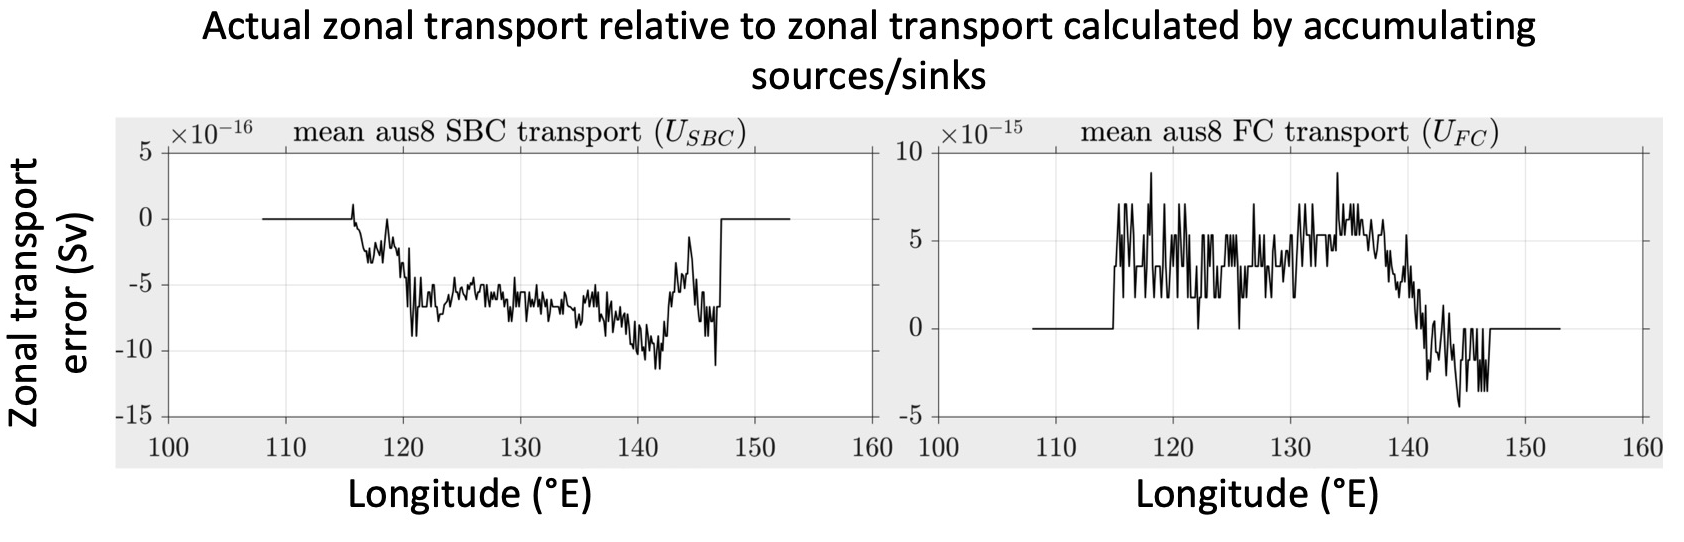
\includegraphics[width=1\textwidth, height=1\textheight, keepaspectratio]{Slide1_2.jpg}
    \caption{\label{Slide1_2}%
    Zonal transport error in Sv for the SBC (left) and the FC (right) showing the differences between the left-hand and right-hand sides of equations (16) and (17).}
\end{figure}

Since the volume budget closes to a high precision, it is evident that the longshore transport across a section can be determined by accumulating the lateral and vertical transports across the faces of the control volume upstream of the section, regardless of the orientation of the section (Fig.2).

\subsection{On using meridional sections rather than normal sections}

The most straightforward orientation of the section is meridional because the section then automatically follows faces of our classical lat-lon gridboxes. Next, we use Fig.\,\ref{slices} to explain the differences between meridional slicings and slicings normal to the coast.

\begin{figure}[hbp]
    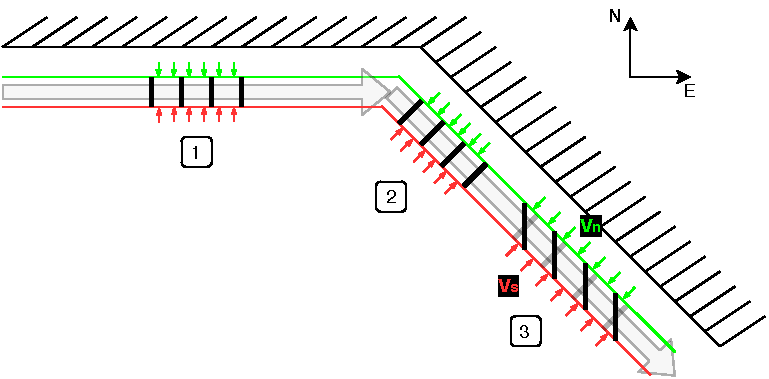
\includegraphics[width=1\textwidth, height=1\textheight, keepaspectratio]{slices.pdf}
    \caption{\label{slices}%
    Simplified schematics of the SBC (wide arrows) along a zonal shelf and a slanted shelf. The SBC is bounded to the north by the green line and to the south by the red line. The thin coloured arrows show the horizontal cross-boundary transports into the SBC across the north face ($V_n$) and south ($V_s$) of the SBC (we assume these transports to be into the SBC for simplicity). There is also an implied vertical transport across the bottom face of the SBC volume which we do not represent here for simplicity. $V_n$ and $V_s$ are the lateral transports across the north and south faces of the current, respectively. The slicing across the SBC volume is shown as thick lines. Case 1 shows meridional slices along a zonal shelf. Case 2 shows normal slices along a slanted shelf. Case 3 shows meridional slices along a slanted shelf (thick black lines) and normal slices along a slanted shelf (thick semi-transparent gray lines).}
\end{figure}

\subsubsection{On the difference between the zonal transport and the longshore transport}

Where the shelf is oriented zonally (Case 1 in Fig.\,\ref{slices}), the meridional slices are normal to the coast. If we were to slice the volume perpendicularly to the slanted coast (Case 2 Fig.\,\ref{slices}), this would result in a situation equivalent to Case 1. In Case 3 of Fig.\,\ref{slices}, meridional slices along the slanted coast (thick black lines) are longer than if they were normal to the coast (thick gray lines). Despite this difference, the volume transports across the two slices can be different only by lateral inflows across the sides of the little triangles formed by these two slices and by the vertical transports across the bottom faces of the triangles as shown below. In Fig.\,\ref{slices} and in the below equation we only consider the lateral inflows for simplicity.

If $\mathcal{\hat{U}}$ is the transport across the meridional slices and $\mathcal{U}$ is the transport across the slices normal to the coast, then

\begin{equation} \label{eq:20}
\mathcal{\hat{U}} = \mathcal{U} + V_{n}dl_{n} - V_{s}dl_{s},
\end{equation}
%
where $V_{n}$ is the inflow across the north face of the current (Fig.\,\ref{slices}), $dl_{n}$ is the length along the north face between a meridional slice and a normal slice, $V_{s}$ is the inflow across the south face of the current (Fig.\,\ref{slices}), $dl_{s}$ is the length along the south face between the meridional slice and the normal slice.

Hence, for a given meridional slice, some extra flows across the north face equivalent to $V_{n}dl_{n}$ are included in the current transport and some flows across the south face equivalent to $V_{s}dl_{s}$ are not included in the current transport, in comparison to a normal slice. When the current is wider, $dl_n$ and $dl_s$ become accordingly longer and the difference between $\mathcal{U}$ and $\hat{\mathcal{U}}$ tends to be larger (depending on the signs and sizes of $V_n$ and $V_s$).

\subsubsection{On the difference between zonal transport and longshore transport in the South Australian Current System case}

An implication of the above discussion is that, while it is true that volume transports with meridional slices will be different to volume transports with normal slices where the shelf is slanted, the difference between the meridional slicing and the normal slicing will be minimal provided:
%
\begin{itemize}
    \item that the slant is not too meridional. If the slant is too meridional, the sides of the little triangles (Case 3 in Fig.\,\ref{slices}) rapidly grow and the two volume transports ($\mathcal{U}$ and $\hat{\mathcal{U}}$) diverge; and
%
    \item that the currents are narrow. If the currents are too wide, the sides of the little triangles will also be too long.
\end{itemize}

In Fig.\,\ref{screenshot} we show a faded, zoomed-in version of Fig.\,3c where we added meridional and normal slices for the FC in a few selected regions. We can see that the triangles resulting from the tilt difference between meridional and normal slices increase in size where the current is wider (e.g.~western most slices) and where the slant is stronger (e.g.~eastern most slices). Given the narrowness of the SBC, the difference between meridional slices and normal slices will be minimal and is not shown in the figure. For the FC, there may be some local differences where the current gets wider or where the slant is stronger (west of Tasmania). These local differences are acceptable because in this paper we do not try to make precise comparisons of our transport values with other estimates at each point for the FC or SBC. Rather we intend to show how these currents' transports vary along the coast. Unless we compare our transport values directly with cross-shore observations, the difference $\mathcal{\hat{U}} - \mathcal{U} = V_{n}dl_{n} - V_{s}dl_{s}$ is immaterial because our volume budget analysis is self-consistent and leak-free. For all the reasons discussed above, we used the zonal transport for the transport of the currents.
%
\begin{figure}[tbhp]
\centering
    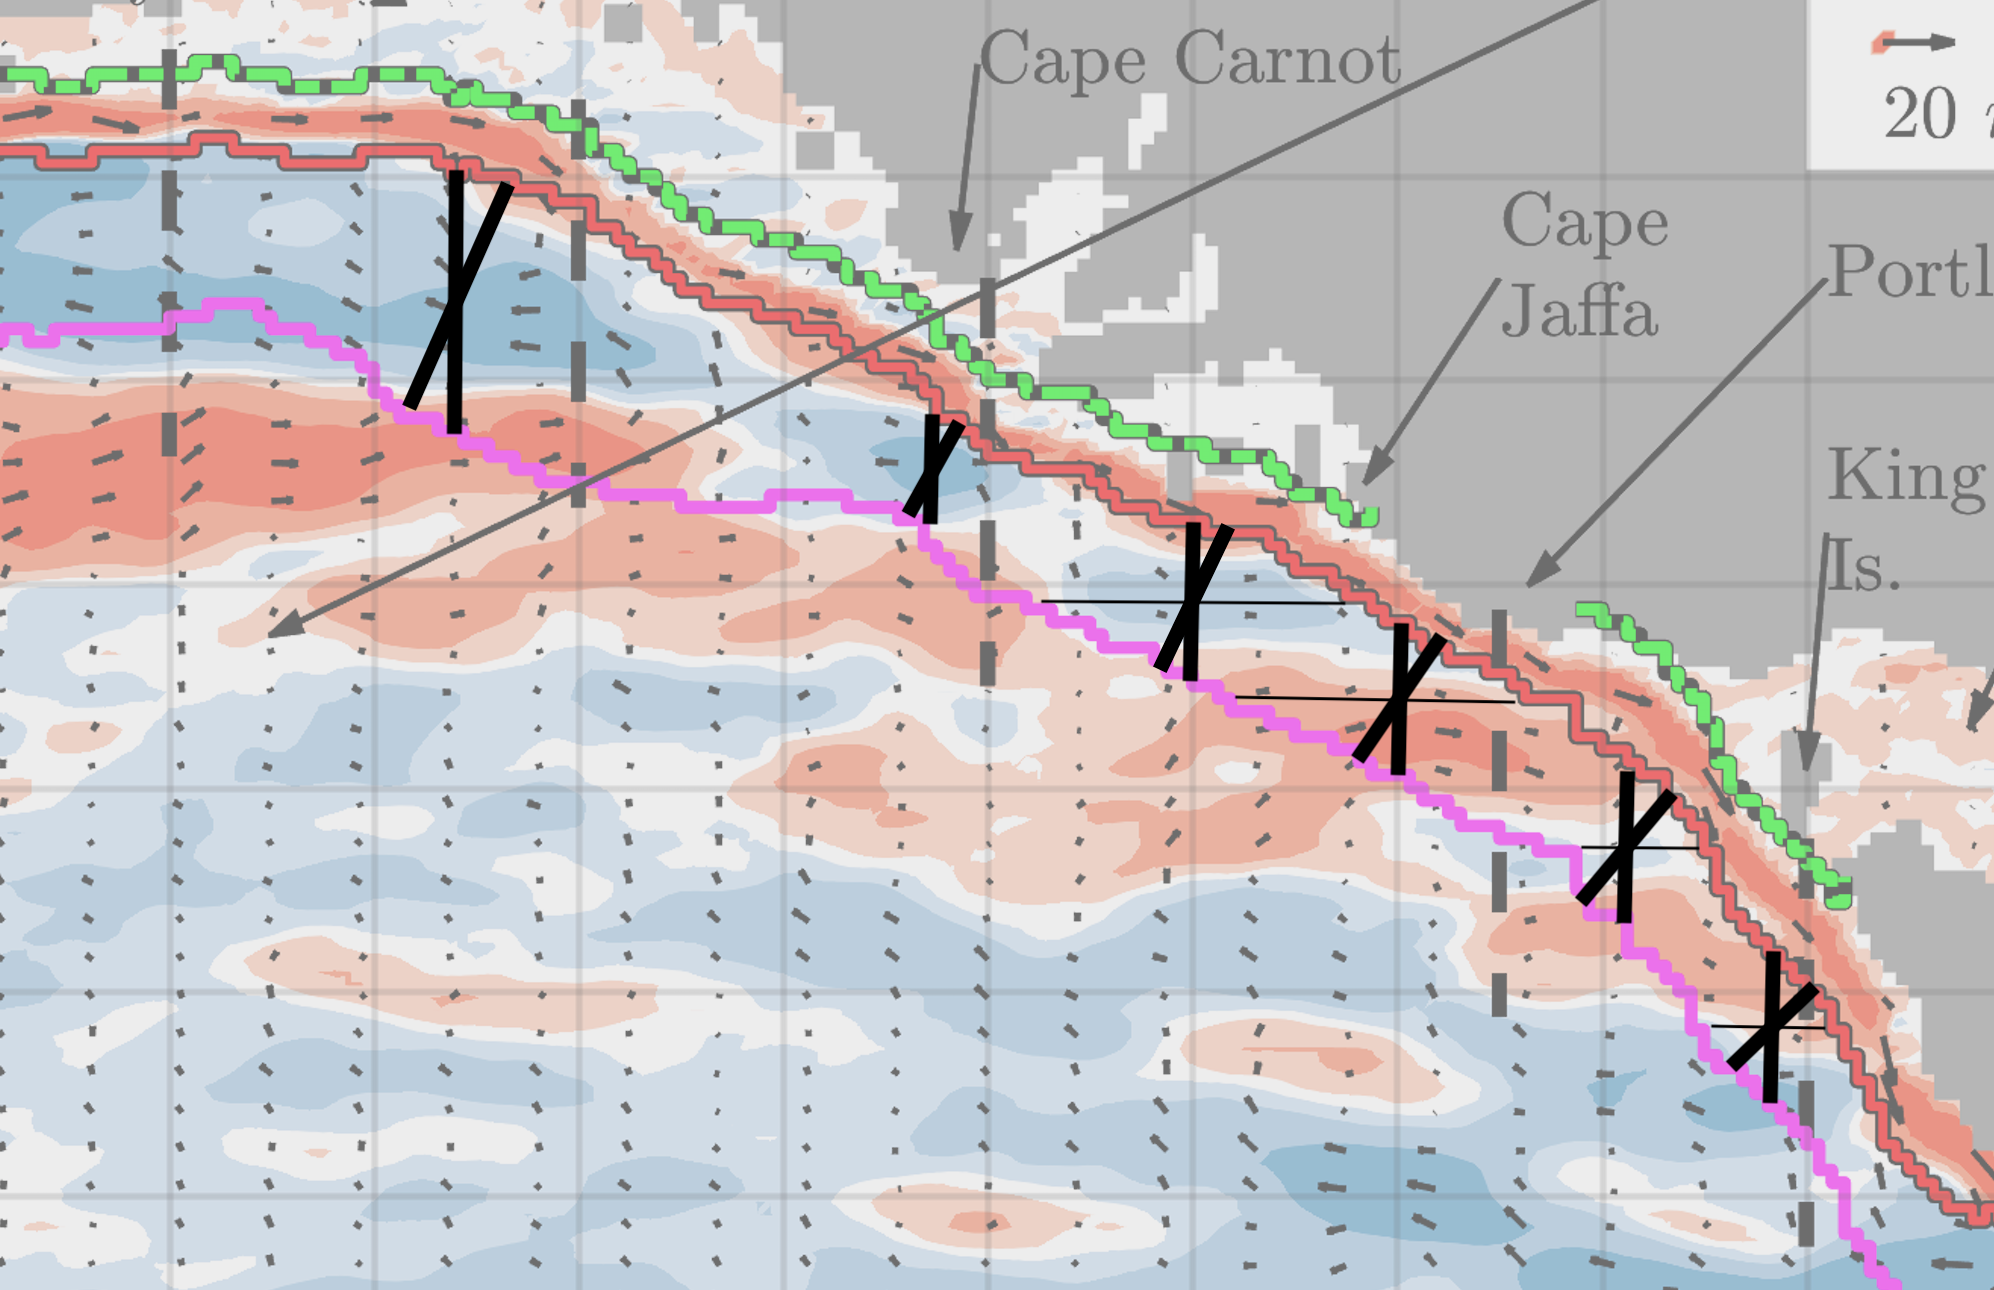
\includegraphics[width=0.8\textwidth, keepaspectratio]{screenshot_copy.png}
    \caption{\label{screenshot}%
    Faded and zoomed-in version of Fig.\,3c. Some examples of meridional and normal slices are shown as thick black lines. The difference between meridional slices and normal slices is shown by the triangles resulting from the tilt difference between the two slices. Zonal slices where the shelf is more slanted are shown as thin black lines. The normal slices are drawn by eye for illustrative purposes.}
\end{figure}

Even if we wanted to calculate a transport like $\mathcal{U}$ above, defining a cross-shore section is not straightforward given that the coast line is not a smooth curve. Then, if all sections follow outlines of grid-boxes, leak-free calculations are feasible, but in this case, each section would have to be defined manually. If, on the other hand, the sections are allowed to intersect grid-boxes, remapping the velocity field in such a way that the total volume is conserved would be very difficult and beyond the scope of this work. 

\clearpage
\bibliographystyle{agufull08.bst}
\bibliography{references.bib}
\end{document}

